% !Mode:: "TeX:UTF-8"
%!TEX program  = xelatex

%\documentclass[bwprint,fontset=windows]{gmcmthesis}
\documentclass[bwprint]{gmcmthesis}
\usepackage{longtable}
\usepackage{graphicx}
\usepackage{epstopdf}
\usepackage{diagbox}
\usepackage{tabularx}
\usepackage{listings}
\lstset{
	numbers=left, 
	numberstyle= \tiny, 
	keywordstyle= \color{ blue!70},%设置关键字颜色
	commentstyle= \color{red!50!green!50!blue!50}, %设置注释颜色
	frame=shadowbox, % 阴影效果
	rulesepcolor= \color{ red!20!green!20!blue!20} ,
	escapeinside=``, % 英文分号中可写入中文
	xleftmargin=2em, %距离左边界2em
	aboveskip=1em,
	framexleftmargin=2em,
	basicstyle=\ttfamily,
	columns=fullflexible,%可以自动换行
	linewidth=1\linewidth, %设置代码块与行同宽
	breaklines=true,%在单词边界处换行。
	showstringspaces=false, %去掉空格时产生的下划的空格标志, 设置为true则出现
	breakatwhitespace=ture,%可以在空格处换行
	escapechar=`%设置转义字符为反引号
}




\hypersetup{hidelinks}
\usepackage[framemethod=TikZ]{mdframed}
\usepackage{array} % 在导言区引入 array 包
\usepackage[UTF8]{ctex} % 加载支持中文的ctex包
\usepackage{amsmath} % 加载amsmath包以支持更复杂的数学公式

%\usepackage{fontspec}  % for Consolas & Courier New
%\lstset{basicstyle=\small\fontspec{Consolas}}
%\lstset{basicstyle=\small\fontspec{Courier New}}
%\setmonofont{Consolas}
%\setcounter{tocdepth}{3}   % 调整目录深度
\usepackage{booktabs}
\usepackage{subfig}
\usepackage{colortbl}
\definecolor{color1}{rgb}{0.78,0.88,0.99}
\definecolor{color2}{rgb}{0.36,0.62,0.84}
%\definecolor{color3}{rgb}{0.8235,0.8706,0.9373}
\definecolor{color3}{rgb}{0.88,0.92,0.96}
\definecolor{color4}{rgb}{0.96,0.97,0.98}%{0.9176,0.9373,0.9686}

% 算法
\usepackage[noend]{algpseudocode}
\usepackage{algorithmicx,algorithm}
\floatname{algorithm}{算法}
\renewcommand{\algorithmicrequire}{\textbf{输入:}}
\renewcommand{\algorithmicensure}{\textbf{输出:}}

%\numberwithin{equation}{section}
%\numberwithin{figure}{section}
%\numberwithin{table}{section}
\newcommand{\red}[1]{\textcolor{red}{#1}}
\newcommand{\blue}[1]{\textcolor{blue}{#1}}


%===================== 建模论文题目 ======================

\title{基于WLAN组网中网络吞吐量的精准建模}
\baominghao{\hspace{6em} 24102860070} %参赛队号
\schoolname{\hspace{5.8em} 华南师范大学}%学校名称
\membera{\hspace{6em} 曾文泉} %队员A
\memberb{\hspace{6em} 蔡镛任} %队员B
\memberc{\hspace{6em} 刘时宇} %队员C

%=======================================================


\begin{document}

 %生成标题
\maketitle

 %填写摘要
\begin{abstract}

本研究针对无线局域网(WLAN)在同频组网环境中的性能挑战,特别是同频干扰或共信道干扰(CCI)对网络性能的影响,提出了基于实测数据的特征构建和分析方法,进一步训练Stacking集成学习模型,实现了对WLAN系统吞吐量的精确预测,克服了传统仿真模型在实际部署中的局限性。


针对问题一,首先对\textbf{数据预处理},选取合适的参数作为特征值进行\textbf{相关性分析}。本文发现RSSI相关参数对AP发送机会具有较高影响但特征维度较大,因此基于RSSI,进一步构建\textbf{信干噪比(SINR)}和\textbf{信号质量(Sq)}两类指标实现降维。同时,结合强弱影响排序,选取\textbf{5类特征值}(在训练集中变量名为:SINR、protocol、sq、per和eirp),构建\textbf{Stacking集成学习}模型。通过交叉验证和网格搜索,获取最优化参数。最终,2个AP测试集上的R\textsuperscript{2}为\textbf{0.98},均方根误差仅为\textbf{1.45};3个AP测试集上的R\textsuperscript{2}为\textbf{0.94},均方根误差仅为\textbf{2.75}。实现了对AP发送机会的高精度预测。

针对问题二,考虑到MCS和NSS为分类变量,且样本比例极不均衡。结合问题一,在深入分析训练集中各参数与MCS和NSS的相关性后,发现MCS与5个变量的相关性均大于\textbf{0.5},包括变量erip、SINR和Sq。而NSS仅与MCC有较强相关性,约为0.4。因此,本文构建了\textbf{层次预测模型},首先预测上层目标变量MCS,将预测结果作为输入特征,进一步预测下层目标变量NSS。在进行下层预测时,考虑到NSS变量的\textbf{长尾分布特征},提出\textbf{Kmeans聚类欠采样}和\textbf{SMOTE过采样方法},解决样本不均衡问题。然后对模型通过交叉验证和网格搜索,获取最优化参数。最终,上层MCS测试集的Recall为\textbf{0.81},F1分数为\textbf{0.80};下层NSS测试集的Recall为\textbf{0.92},F1分数为\textbf{0.92}。进一步对模型的性能评估,证实了该模型在上层特征提取和下层样本分类方面能力显著,实现了对(MCS,NSS)更优的预测结果。

针对问题三,首先分析对系统吞吐量有影响的变量,主要分析了随机回退机制,得到了$CW_{min}=6$ 下,2个AP下的随机回退时间期望,还分析了数据帧聚合机制对于吞吐量的影响,确定使用层次 stacking 预测模型,实现两次级联完成新特征对吞吐量的预测。对模型通过交叉验证和网格搜索,获取最优化参数。最终,该模型整体的R\textsuperscript{2}为\textbf{0.91},平均绝对误差(MAE)为\textbf{11.9}。然后对模型进行评估,证实了该模型对WLAN吞吐量的高精度预测。

\keywords{无线局域网; 吞吐量; 集成学习; 层次预测; 重采样}

\end{abstract}

\pagestyle{plain}

%目录 不推荐加
\maketoc

\clearpage

\section{问题重述}

\subsection{问题背景}   % 问题的背景

无线局域网(WLAN)已成为现代通信基础设施不可或缺的一部分,尤其是在需要灵活移动连接的场景下。在密集部署的环境中,同频组网作为一种实现零漫游的组网方式,被广泛应用。在这种配置下,各个AP之间的干扰成为了一个显著的问题,特别是同频干扰或共信道干扰(CCI),它会导致数据包丢失、重传增加、网络覆盖范围缩减以及连接不稳定等问题,从而严重影响了WLAN的性能和服务质量。

然而,传统的基于仿真的模型在实际部署中往往无法达到预期的效果,因为现实世界中的WLAN通信面临着信道条件快速变化、多种干扰源以及复杂的服务流量等问题。因此,本研究致力于基于实际测量数据,深入分析同频AP环境下的各种影响因素,如网络拓扑、RSSI、信道接入机制及同频干扰等,从而实现更为精确的吞吐量预测。通过这种方式,我们期望能够提出一种更贴近实际应用需求的优化方案,以改善WLAN系统的性能表现。

本研究旨在基于WLAN的同频组网实测数据,分析网络拓扑、节点间RSSI、信道接入机制、干扰等因素对数据传输速率的影响,进而实现对WLAN系统吞吐量的精确预测。通过该预测模型对WLAN系统进行优化,有望在工业、教育、医疗等新兴场景中实现突破,为用户提供卓越的业务体验。

\subsection{问题描述}
\subsubsection{问题一}
首先根据附件WLAN网络实测训练集中所提供的网络拓扑、业务流量、门限、节点间RSSI的四类测试基本信息,分析其中各参数对AP发送机会的影响,并给出影响性强弱的顺序。并且通过训练的模型,预测每个AP的发送机会或是概率,即发送数据帧序列的总时长(seq\_time),并通过测试集 test\_set\_1\_2ap和test\_set\_1\_3ap预测AP发送数据帧序列的总时长。可按照同频AP个数分类分析和分别建模,也可统一分析和建模。

其中包含三个任务:第一个任务为利用训练集中提供的四类测试基本信息对AP发送机会的影响强弱进行判断并排序。第二个任务为利用训练集进行训练,预测AP发送的机会,即发送数据帧序列总时长;第三个任务为利用训练好的模型对两个测试集进行AP发送数据帧序列的总时长。

为了分析WLAN网络中各参数对AP发送机会的影响并建立相应的预测模型,我们首先依据提供的网络拓扑、业务流量、门限及节点间RSSI这四类基本信息,评估这些参数对AP发送机会的具体影响,并确定各个因素影响的强弱顺序;随后,使用训练集中的数据进行模型训练,以预测每个AP的发送机会,具体表现为发送数据帧序列的总时长(seq\_time);最后,运用训练好的模型对两个特定的测试集(test\_set\_1\_2ap 和 test\_set\_1\_3ap)进行预测,确定在不同数量的同频AP环境下AP发送数据帧序列的总时长。整个过程既可以通过按同频AP的数量分类分析和分别建模的方式进行,也可以采取统一分析与建模的方法,以确保模型能够准确反映实际情况并提供可靠的预测结果。

\subsubsection{问题二}
根据附件提供的实测训练集中的问题1中提到的四类测试基本信息,特别是节点间RSSI信息和门限信息,结合问题1中对AP发送机会的分析,对测试中AP发送数据选用最多次数的(MCS, NSS)进行建模,并通过测试集 test\_set\_2\_2ap和test\_set\_2\_3ap预测(MCS, NSS)。

AP在自适应调制与编码AMC算法下自适应调节发送速率,AP通过监测信道条件SINR信干燥比的大小,在过程中动态地采用多个(MCS, NSS),为了使AMC算法收敛速度快,故其中选用最多次数的(MCS, NSS)代表了此组合下是当前信道的最佳组合。

在WLAN网络中,AP通过自适应调制与编码(AMC)算法根据信道条件(如SINR)动态调整发送速率,选择使用次数最多的(MCS, NSS)组合作为当前信道的最佳组合,要求根据训练集中的网络拓扑、业务流量、门限信息、特别是节点间RSSI信息,分析这些参数对AP发送机会的影响,找出与MCS和NSS相关性较高的特征值,并基于这些特征值训练模型预测在给定信道条件下AP最常选用的(MCS, NSS)组合,最终使用训练好的模型对两个测试集(test\_set\_2\_2ap 和 test\_set\_2\_3ap)进行预测,得到AP最常选用的(MCS, NSS)组合。

\subsubsection{问题三}
结合问题1和问题2的分析,对系统吞吐量进行建模,并通过测试集test\_set\_1\_2ap和test\_set\_1\_3ap预测网络吞吐量。无线信道具有瞬息万变的特点,实测中所测量的RSSI信息属于大尺度信息,不足以完全反应真实信道变化,因而问题2对(MCS, NSS)的建模可能无法获得很高精度。允许采用实测中统计的数据帧真实(MCS, NSS)作为模型输入变量。在题目的基础上,不仅需要结合前两文的内容,对于问题2的MCS、NSS放入模型,还要从题干中提取新的特征值完成模型的训练。


\section{问题分析}
\subsection{针对问题一的分析}

问题1的处理首先要建立在数据的高质量预处理上,将问题中给出的四类测试基本信息选出合适的相应指标作为特征值进行相关性分析或训练。分析其对AP发送机会的影响,若参数对AP发送机会重要性强,那么AP 发送受其影响则更大,则AP发送数据帧序列总时长(seq\_time)将会变短;反之参数若对AP发送机会干扰弱,那么AP发送的概率或次数将增大增多,则AP发送数据帧序列总时长将会边长。

给出的数据中RSSI数值数量较多且不宜直接应用,应先对RSSI进行处理,并通过题目中给出的关系,尽可能构建对AP发送数据帧序列总时长相关的新特征,可以更好的在后续的模型训练中得到更大的贡献值。对所有特征值指标对seq\_time指标完成相关性分析后,可以通过机器学习模型训练反过来排列对seq\_time指标影响的重要度排名对相关性分析进行一定的校准与验证,最后利用相关度较高的特征,对seq\_time指标进行预测模型的训练并完成测试集的预测任务。

\subsection{针对问题二的分析}
由于不同数据处在不同数量的BSS下,其可被影响的AP 数量也不同,在需要预测的数据中也是不同个数AP数据,故可按照同频AP个数分类建模。但对不同AP个数进行统一建模也可以进行训练与预测完成问题的任务,所以为了更好地确认分类建模效果好还是统一建模效果好团队预将三个模型训练效果进行对比,以确保模型地高精度。

\subsection{针对问题三的分析}


\section{模型假设与符号说明}
\subsection{模型的假设}
\begin{assumption}
	\label{asm:1}
	数据中包括的三个AP均处在同一信道中,即属于同频AP,节点之间发送数据会造成相互干扰与影响且属于同频干扰;
\end{assumption}

\begin{assumption}
	\label{asm:2}
	假设在场景中AP或STA接受数据时收到的环境底噪较小,忽略不计,干扰均来自于其他AP或STA传输的数据;
\end{assumption}

\begin{assumption}
	\label{asm:3}
	假设TCP协议在本题中不考虑三次握手和四次挥手建立连接过程,即只考虑数据传输过程;
\end{assumption}

\begin{assumption}
	\label{asm:4}
	假设在场景中只存在同频干扰,不存在异频干扰,且相邻AP不进行通信。
\end{assumption}

\subsection{主要符号说明}
\subsubsection{缩略字母说明,其他缩略字母请见正文部分}

\begin{table}[H]
	\centering
	\caption{缩略字母说明}
	\begin{tabular}{p{2.0cm}<{\centering}p{8.0cm}<{\centering}p{4.0cm}<{\centering}}
		%指定单元格宽度, 并且水平居中。
		\hline
		缩略字母 & 全称 & 中文含义  \\ %换行 
		\hline
		$AP$ & Access Point & 无线接入点   \\ %把你的符号写在这
		STA	& Station	& 站点\\
		
		RSSI &	Received Signal Strength Indication	& 接收信号能量强度\\
		
		WLAN &	Wireless Local Area Network	& 无线局域网\\
		
		CCA &	Clear Channel Assessment	& 信道可用评估\\
		
		PD &	Packet Detection	& 包检测门限\\
		
		ED &	Energy Detection	& 能量检测门限\\
		
		NAV	 & Network Allocator Vector	& 网络分配矢量\\
		
		SINR &	Signal To Interference And Noise Ratio	& 信干噪比\\
		
		MCS &	Modulation and Coding Scheme	& 调制编码方案\\
		
		NSS &	Number of Spatial Stream	& 空间流数\\
		
		BSS &	Basic Service Set	& 基本服务集\\
		
		\hline
	\end{tabular}
\end{table}

\subsubsection{参数符号说明}
\begin{longtable}{ c c c }
	\caption{参数符号说明} \\ % 表格标题
	%指定单元格宽度, 并且水平居中。
	\hline
	符号 & 含义   \\ %换行 
	\hline
	
	$d$	& 接收信号的距离\\
	$d_0$ &	接收信号的及基准距离\\
	$ \lambda $	& 路径动态衰减参数\\
	$X_{\theta}$ &	均值为$\sigma$标准差为$\theta$的高斯分布随机函数\\
	$P_s$ &	数据信号的功率值\\
	$P_i$ &	干扰信号的功率值\\
	$P_n$ &	环境底噪的功率值\\
	$RSSI_s$ &	数据信号的接收信号强度\\
	$RSSI_i$ &	干扰信号的接收信号强度\\
	$NAV_i$ &	当前信道i的NAV门限值\\
	$v_i$ &	第i个数据的剩余误差\\
	$ \alpha $ &	同步传输强度占混合传输强度的比例\\
	$\beta_1$ &	信号强度处于PD和ED门限之间的信号中携带preamble前导头的概率\\
	$\beta_2$ &	信号强度超过ED门限的信号中能被准确识别的判断信道繁忙的概率\\
	$C_{HN}$ &	奈奎斯特信道传输速率\\
	$C_{CS}$ &	香农信道传输速率\\
	
	\hline
\end{longtable}

\section{模型准备}
\subsection{WLAN工作流程}

在 AP 或 STA 端,发送和接收数据信号的功能不能同时进行。根据题目要求,本文遵循的端口发送数据和接收信号的流程,如下图所示。

% TODO: \usepackage{graphicx} required
\begin{figure}[H]
	\centering
	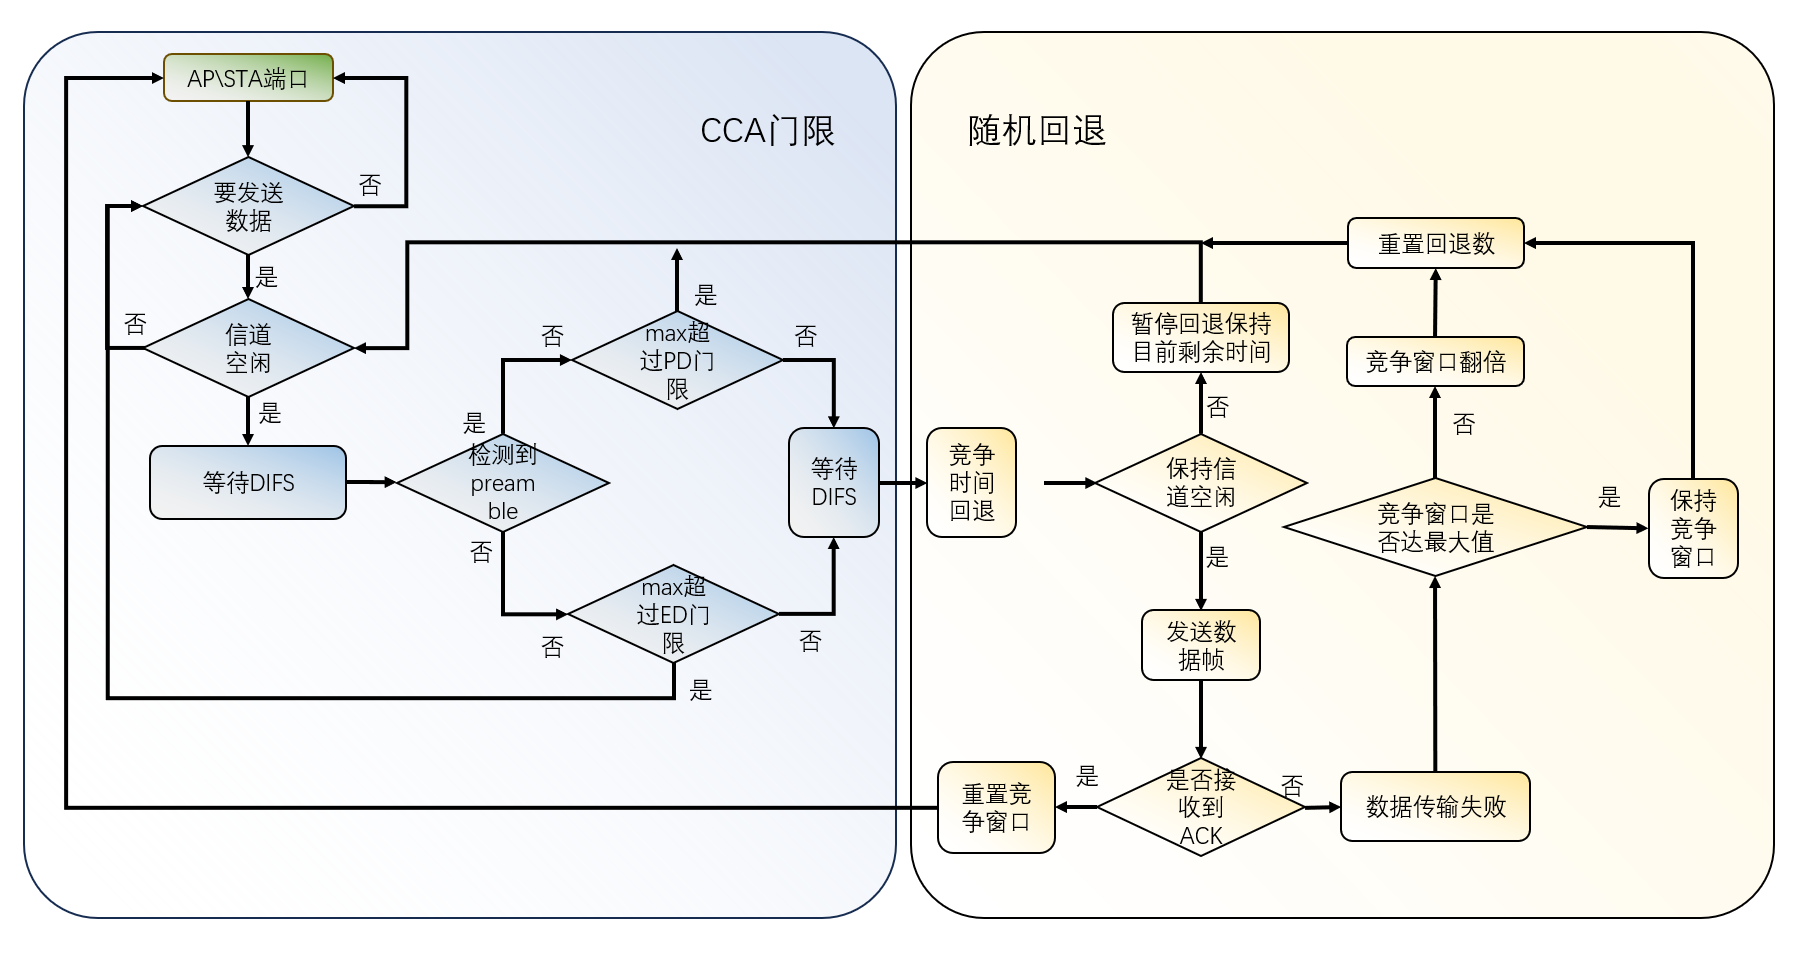
\includegraphics[width=0.9\linewidth]{figures/4.1}
	\caption{端口发送数据流程图}
	\label{fig:端口发送数据流程图}
\end{figure}

图4.1展示了 AP(接入点)在发送数据帧时遵循的基本步骤。此过程涉及 802.11 标准中的竞争窗口(CW)和退避机制,以确保多设备共享同一信道时避免冲突。步骤如下:

\begin{itemize}
	\item 检查是否要发送数据:如果AP有数据需要发送,则进入下一步。
	\item 确保信道空闲:即基于是否处于nav时段确认信道空闲与否或者其他方式确认信道空闲。
	\item 等待 DIFS 时间:AP 等待指定的时间间隔DIFS以确认信道空闲。
	\item 检测 preamble:通过是否错过preambel头选择使PD门限还ED门限判定信道空闲。
	\item 判定PD门限:如果检测到了preamble头,则选择PD门限判定信道空闲,噪声RSSImax超PD门限,说明信道繁忙,返回等待信道空闲。
	\item 判定ED门限:如果未检测到preamble头,则使用ED门限,如果检测到的RSSImax超PD门限),说明信道繁忙,返回等待信道空闲。
	\item 竞争时间回退:如果信道空闲满足发送条件,AP 将从竞争窗口CW随机选择一个竞争时间。如果在此期间信道保持空闲,AP 将发送 RTS 或 CTS 数据帧,来获取信道使用权。
	\item 暂停回退:如果收到 CTS,AP 暂停回退计数器并保持当前剩余时间。
	\item 发送数据帧:如果信道保持空闲且回退时间到0,AP 发送数据帧。
	\item 接收到 ACK:如果成功发送数据帧并接收到确认帧(ACK),则结束发送过程。
	\item 竞争窗口翻倍:发送结束等待超时,长时间未受到ACK确认帧,则会使得CW增大,即在窗口未达到CWmax情况下CW翻倍,重新进行随机回退机制。
\end{itemize}

综上,该流程图展示了 CSMA/CA(载波监听多路访问/冲突避免)协议在无线局域网中的运作,以防止数据帧冲突。当信道繁忙时,设备会退避一段时间后再尝试发送,而在发生冲突时,设备会增大竞争窗口,减少再次冲突的可能性。

% TODO: \usepackage{graphicx} required
\begin{figure}[H]
	\centering
	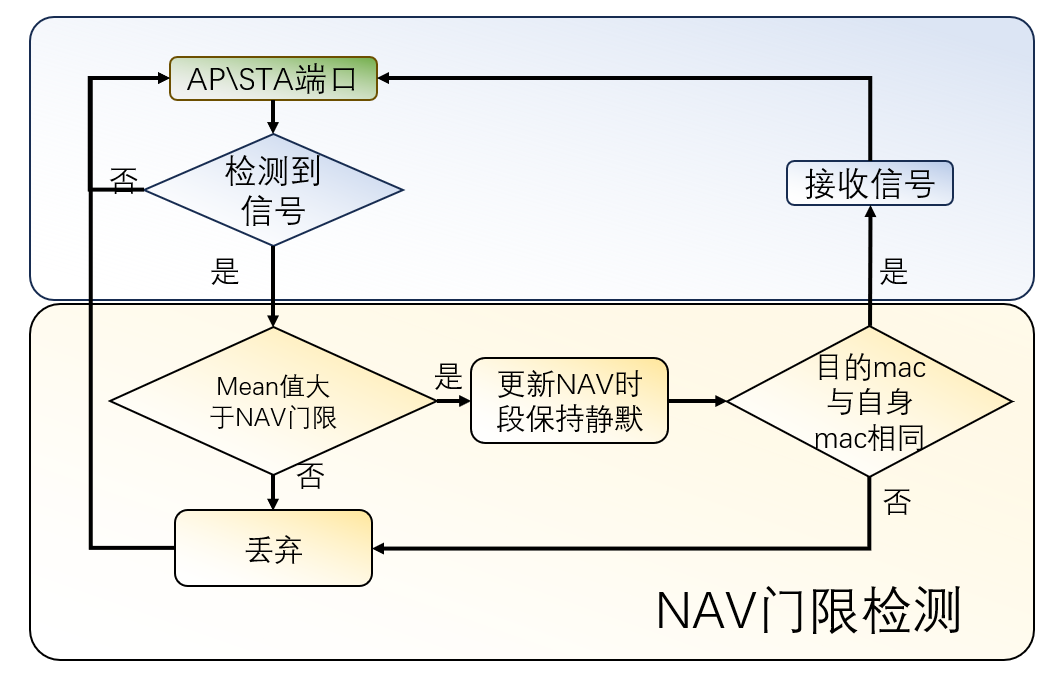
\includegraphics[width=0.7\linewidth]{figures/4.2}
	\caption{端口接收数据流程图}
	\label{fig:端口接收数据流程图}
\end{figure}

图4.2展示了一个简单的无线设备(如AP或STA)在接收信号时的过程。在这个过程中,设备首先判断是否有信号到达,然后根据信号的情况决定是否接收或丢弃信号。具体步骤如下:

\begin{itemize}
	\item AP/STA端口:设备从端口获取信号。
	\item 检测信号:设备检查是否有信号输入。
	\item Mean值与NAV门限比较:若检测到信号,计算其平均值(Mean值)并与NAV门限比较。若Mean值小于或等于NAV门限,设备将忽略该信号。
	\item 更新NAV时段:若Mean值大于NAV门限,设备更新NAV时段,并保持静默状态,停止发送数据以便其他设备发送。
	\item 接收信号:如果Mean值大于NAV门限,设备继续接收信号。
	\item 目的MAC地址匹配:检查信号的目的MAC地址是否与自身相同。若相同,继续处理该信号;若不同,设备将丢弃该信号。
\end{itemize}

综上,本文简化了无线设备在接收信号时的行为,主要关注信号的质量和目的地址的匹配。


\subsection{训练集参数分析}

在了解并对无线设备的发送与接收信号行为流程后,如果预要利用好数据,需要对应题目给出的信息进行训练集中特征的分析,对不同的参数信息有一定的了解,尤其重点关注在题干中出现的信息类别中的数据。


\begin{figure}[H]
	\centering
	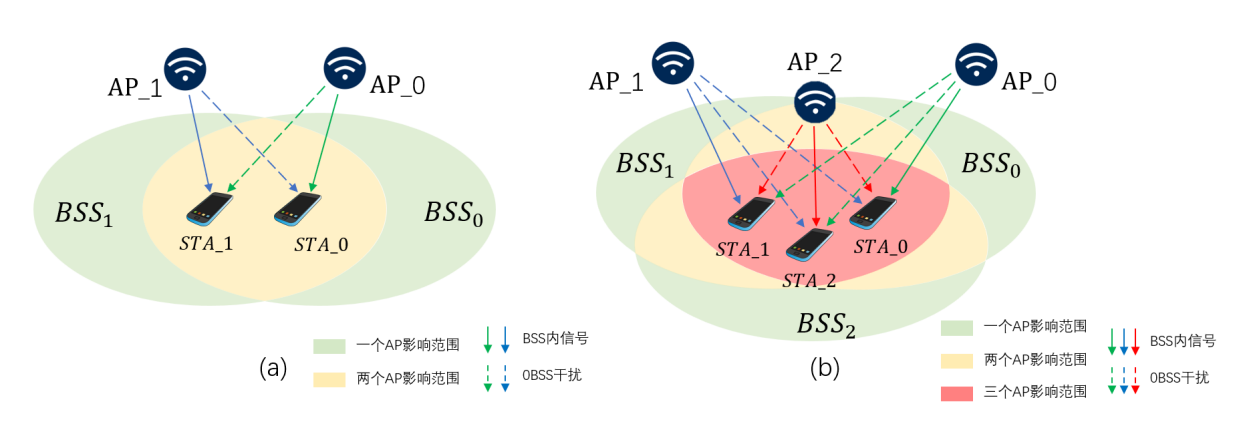
\includegraphics[width=1\linewidth]{figures/阔谱图}
	\caption{WLAN拓扑图}
	\label{fig:}
\end{figure}




\subsubsection{节点间的接收信号强度}

例如题中所提供的网络拓扑图所示,明显网络拓扑中ID内容不会对AP发送机会造成干扰,但其中AP与STA部署的位置将会影响节点间传输的距离,而距离是影响RSSI的重要指标,RSSI参考公式为:

\begin{equation}
	RSSI\left( d \right) =RSSI\left( d_0 \right) +10\lambda \lg \left( \frac{d}{d_0} \right) +X_{\sigma}
\end{equation}

可以发现,距离(d)处接收到的信号强度值(RSSI(d))是以$d=d_0$作为参考的,信号强度随着传播路径的增加,在一个均值为0标准差为$ \theta $ 的高斯分布随机函数($X_{ \theta }$)的基础上以一定的路径动态衰减参数($ \lambda $)为参数的衰减速度递减。所以AP与STA部署的位置会不同程度的干扰AP发送机会。

\subsubsection{业务流量}

业务流量包含数据报协议与数据长度两个方面组成,其中数据报协议类型中UDP与TCP两种不同的协议虽然报文大小相同,但是两种传输协议的连接方式、传输可靠性、流量控制、数据流向是大相径庭的,UDP适用于轻量级、时延敏感但可靠性要求不高的场景,而TCP更适合需要可靠性和数据完整性保障的场景。这就导致不同的传输协议会对AP发送机会造成影响。

在本研究中,针对TCP协议,仅关注数据传输过程而不涉及连接建立过程。根据IEEE 802.11标准,在无线局域网(WLAN)中,不论是TCP还是UDP协议,均可采用单播(unicast)或广播(broadcast)模式进行数据传输。然而,在本研究中,我们专注于单播模式下的点对点传输,即数据包从源节点发送到一个特定的目的节点,并且在这种模式下,当数据接收节点成功接收到数据后,会发送一个ACK确认帧以告知源节点数据已被正确接收。

考虑到TCP协议头部至少为20字节,而UDP协议头部固定为8字节。为了量化不同协议类型的数据处理,我们将把协议头部长度与ACK确认帧的长度结合起来考虑。这样,可以更准确地衡量不同协议在数据传输过程中的开销.

\subsubsection{门限}

门限在其中包括CAA门限中的包检测门限PD和能量检测门限ED以及NAV门限。其中NAV门限用于接收数据帧时,判断是否接收数据帧,PD门限和ED门限用于在发送数据帧时,判断信道是否空闲,具体过程在端口发送数据和接收数据流程图4.1与图4.2中体现。

\subsubsection{节点间RSSI}

在无线局域网(WLAN)的同频组网模式下,节点间的传输方向主要分为三类:无线接入点(AP)与AP之间、AP与站点(STA)之间、以及STA与STA之间。在这种网络架构中,同级别的相邻节点(例如AP与AP或STA与STA)并不直接进行通信,因此它们接收到的数据信号通常被视为干扰噪声。例如,当$AP_0$广播数据信号时,尽管$AP_1$与其相邻并接收到该信号,但在媒体访问控制(MAC)地址验证过程中,若发现目的MAC地址并非自身,则将该信号丢弃,作为干扰噪声处理。同样,不同基本服务集(BSS)内的上下级节点间的通信也被视为干扰噪声。

例如,$AP_0$广播的数据信号被不同BSS内的$STA_1$接收后,同样会在MAC地址验证阶段因不匹配而被丢弃,作为干扰噪声处理。因此,在本研究的二级网络拓扑中,只有ID下标相同的STA和AP之间的数据帧传输信号强度被视为有效信号。

不同节点接收的信号强度指示(RSSI)的总和值(sum)用于计算信干噪比(SINR)。首先,需要对接收到的所有RSSI值进行区分,以判断其是信号还是噪声。随后,根据区分后的信号和噪声计算SINR值。

\subsubsection{信干燥比SINR}

信干燥比是信号功率与干扰加噪声功率之比,直接影响数据传输的可靠性和速率,越高的信干燥比允许使用更高阶的调制编码方案(MCS)和更多的空间流数(NSS)组合,从而提升PHY速率,反之需要降低(MCS,NSS)来保证数据传输的可靠性,故该参数对于预测MCS和NSS组合具有很高参考性。

\subsection{传输速率}

在实际信道传输数据过程中,在奈奎斯特定理和香农定理的双重约束下,信道的时间传输速率不能突破两者上限,其中奈奎斯特定理表示,理想低通信道下的极限数据传输率为信道带宽与码元可承载比特数相关联,由于这个定理只局限在无噪声的环境下计算信道最大数据传输速率,而在有噪声的环境下仍然不能有效计算出信道最大数据传输速率,香农定理将其进一步扩展到了信道受到随机噪声干扰的情况,即在有随机噪声干扰的情况计算信道最大数据传输速率,表明信道的极限数据传输速率与信道带宽与信干燥比相关联,两个定理公式如下。

\begin{equation}
	C_{HN}=2\times W\times \log _2V
\end{equation}
\begin{equation}
	C_{CS}=W\times \log _2\left( 1+SINR \right)
\end{equation}

其中W表示信道带宽,V表示码元可承载比特数。而码元可承载比特数与题中给到的MCS数值大小有关,根据资料显示,不同MCS大小对应不同的调制解调方案,对应着不同的编码率,则其每个码元可以承载的比特数也不相同,故PHYRate与MCS数值有关。而NSS则理论上与PHYRate成正比,但是实际中受到噪声影响,更大的PHYRate则意味着面临更大的干扰,故并非完全正比,题中所给的MCS和NSS组合对应的PHYRate如表4.3所示:

\begin{center}
	\begin{table}[htbp]
		\caption{MCS\$NSS与PHY Rate对应表} \label{tab:mcs_nss_rate} 
		\begin{tabularx}{\textwidth}{|l|*{12}{>{\centering\arraybackslash}X|}}
			\hline
			\diagbox{NSS}{Rate}{MCS} & 0 & 1 & 2 & 3 & 4 & 5 & 6 & 7 & 8 & 9 & 10 & 11 \\
			\hline
			1 & 8.6 & 17.2 & 25.8 & 34.4 & 51.6 & 68.8 & 77.4 & 86.0 & 103.2 & 114.7 & 129.0 & 143.4 \\
			\hline
			2 & 17.2 & 34.4 & 51.6 & 68.8 & 103.2 & 137.6 & 154.9 & 172.1 & 206.5 & 229.4 & 258.1 & 286.8 \\
			\hline
		\end{tabularx}
	\end{table}
\end{center}

\subsection{RSSI均值公式}

RSSI数值是功率P的对数值,因此对RSSI的加减操作本质上对应于功率P的乘除运算。求RSSI的均值,实际上应该是对功率P求均值。本研究推导了适用于计算RSSI的sum列表均值的公式,该推导过程虽可一步得到,但是理解过程对于实际计算RSSI均值的过程具有显著帮助,可用于估算信号强度的大小。

由于RSSI表示的是一种对数关系,直接对RSSI进行合并并不恰当。通过查阅相关资料,可以得知RSSI与功率P之间的转换公式为:

\begin{equation}
	RSSI\left( dbm \right) =10\times \log _{10}\left( \frac{P\left( m,w \right)}{1\left( m,w \right)} \right) 
\end{equation}

其中1(m,w)表示在1m处测量的功率值作为参考,那么可以得到功率P求解公式为:

\begin{equation}
	P\left( m,w \right) =10^{\frac{RSSI\left( dbm \right)}{10}}\times 1\left( m,w \right) 
\end{equation}

则对于RSSI数据组对其进行功率转换后均值处理得到一个信号平均功率:

\begin{equation}
	\overline{P\left( m,w \right) }\ =\ \frac{1}{n}\sum_{i=1}^n{P_i\left( m,w \right)}
\end{equation}

最后可以利用信号平均功率计算得到接受信号平均强度:

\begin{equation}
	\overline{RSSI\left( dbm \right) }=10\times \log _{10}\left( \frac{\overline{P\left( m,w \right) }}{1\left( m,w \right)} \right) 
\end{equation}

\subsection{数据预处理}
\subsubsection{冗余数据处理}

数据文件中给予了许多特征,其中很多特征信息重复冗余,例如bss\_id 、 ap\_id、ap\_mac、sta\_mac和sta\_id这些特征完全对应,仅保留一项ap\_id。

\subsubsection{RSSI数据嵌入策略}

由于采样的随机性,数据采集过程中剔除了一些异常值导致RSSI数据的长度不同,且因此失去了RSSI的sum、max和mean数据的对应性,将使用已知采样数据估计真实数据。对于RSSI的sum、max和mean将采用不同的数据嵌入策略,将高维RSSI数组进行数据嵌入,最终统一的数值。
对于RSSI的sum列表数值,将采取求均值操作,对于一个sum列表,采用RSSI求均值方法,因为异常值对其影响巨大,一个较大的异常值,会覆盖所有正常值,本研究采用基于高斯分布的拉依达法则对异常值进行剔除,以提高数据的准确性。若单元格中存在某一次收集RSSI数值的剩余误差大于了该单元格内测量的RSSI数值的3倍标准差,则认为该RSSI数值应予剔除,然后使用RSSI求均值方法,求其均值,该方法在模型准备中介绍。

如下图所示,将位于[μ-3σ,u+3σ]外的异常值剔除。

\begin{figure}[H]
	\centering
	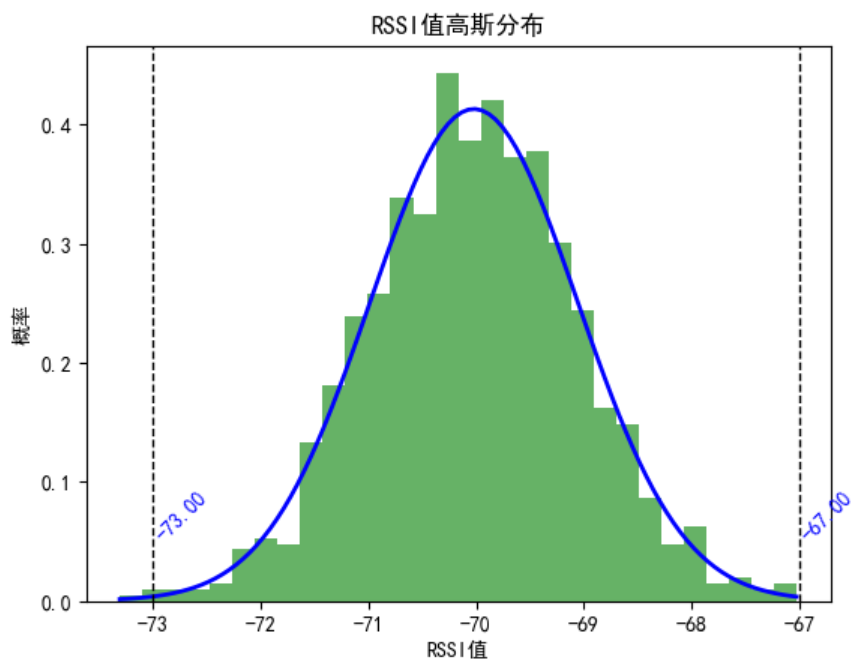
\includegraphics[width=0.7\linewidth]{figures/4.3}
	\caption{RSSI值高斯分布图}
	\label{fig:RSSI值高斯分布图}
\end{figure}

对于max列表数据,使用PD门限和ED门限,求其通过两个门限的通过率,再进行加权求均值,因为ED门限较高,通过较为困难,且通过后抢占信道概率更大,故本研究将PD门限通过率权重为2/3,ED门限通过率权重为1/3。最终得到一个通过率,公式如下所示:

\begin{equation}
	PD\left( RSSI_{max} \right) =\left\{ \begin{array}{l}
		\begin{matrix}
			0&		RSSI_{max}<PD\\
		\end{matrix}\\
		\begin{matrix}
			1&		RSSI_{max}\ge PD\\
		\end{matrix}\\
	\end{array} \right. 
\end{equation}

\begin{equation}
	ED\left( RSSI_{max} \right) =\left\{ \begin{array}{l}
		\begin{matrix}
			0&		RSSI_{max}<ED\\
		\end{matrix}\\
		\begin{matrix}
			1&		RSSI_{max}\ge ED\\
		\end{matrix}\\
	\end{array} \right. 
\end{equation}

\begin{equation}
	Rate_{max}\left( RSSI_{max} \right) =\frac{1}{n}\sum{\left( Wt_{PD}\times PD\left( RSSI_{max}i \right) +Wt_{ED}\times ED\left( RSSI_{max}i \right) \right)}
\end{equation}
\\
最终将数组高维数据降维成一个数。而对于mean列表,以同样的道理,对其使用NAV门限进行计算其通过率,公式如下所示。

\begin{equation}
	NAV\left( RSSI_{mean} \right) =\left\{ \begin{array}{l}
		\begin{matrix}
			0&		RSSI_{mean}<NAV\\
		\end{matrix}\\
		\begin{matrix}
			1&		RSSI_{mean}\ge NAV\\
		\end{matrix}\\
	\end{array} \right. 
\end{equation}

\begin{equation}
	Rate_{mean}\left( RSSI_{mean} \right) =\frac{1}{n}\sum{\left( NAV\left( RSSI_{mean}\_i \right) \right)}
\end{equation}

\subsubsection{传输协议类型数据处理策略}

一次传输过程,由于 TCP 协议头至少为 20byte,UDP 协议头至少为 8byte,所以使用 TCF协议将多花费 20byte,UDP 协议将多花费 8byte。在本题中,无论 UDP 还是 TCP 协议考虑的都是 unicast 模式进行点对点传输数据,每一次传输都需要加上IP协议头且接收节点都会回复 ACK 确认帧,故考虑将数据中的TCP和UDP类别分别替换为20和8,单位为byte,即用协议头花销替代协议类型数据,以达到量化TCP和UDP类别差异。

\subsubsection{分离信号噪声}

在模型准备阶段,本研究已经介绍了如何区分来自不同节点的RSSI信号和噪声。因此,在信号预处理的最后阶段,首先需要对接收自所有节点的RSSI信息进行分离,以区分信号和噪声。在本研究中,信号数据仅存在于上下级节点间的传输中,而接收自其他节点的信息则被视为噪声。
在2AP的情况下,AP仅将与其下级节点STA之间的RSSI数据视为可靠信号,其他节点的RSSI数据则被视为噪声。STA也遵循相同的规则。这一规则同样适用于3AP的情况。

首先对RSSI指标进行优化,在2个AP作用场景中,每两行数据表示在同一次传输数据过程中发送端与接收端相关特征,其中含有多个RSSI相关特征,但对于每一行本身的端口来说,划分为指向性端口对他本身的传输信号RSSI与其他端口对他的干扰信号RSSI,由于是发送端、接收端轮流排列,则导致这一列RSSI中接收到的信息为其他发送端产生的干扰、向本接收端发送的信号轮流排列,而在与之对应的另一列RSSI中,则与之完全相反,呈现出来某一行前后对应的两列数据一个为信号RSSI,一个为其他发送端产生的干扰,为了增加数据特征的表现性与特征显著性,将对应的混乱的两列转化为信号RSSI列和干扰RSSI列。


\section{问题一分析与求解}
\subsection{相关性分析}\label{问题一分析}

本节首先使用Pearson correlation,初步分析各参数对AP发送机会(seq\_time)的影响,为预测模型做准备。(数据来源:第4节预处理后的训练集)。


\begin{equation}
	\small
	\rho_{X, Y} = \frac{\operatorname{cov}(X, Y)}{\sigma_{X} \sigma_{Y}} = \frac{E(X Y) - E(X) E(Y)}{\sqrt{E(X^{2}) - E^{2}(X)} \sqrt{E(Y^{2}) - E^{2}(Y)}}
\end{equation}


% TODO: \usepackage{graphicx} required
\begin{figure}[H]
	\centering
	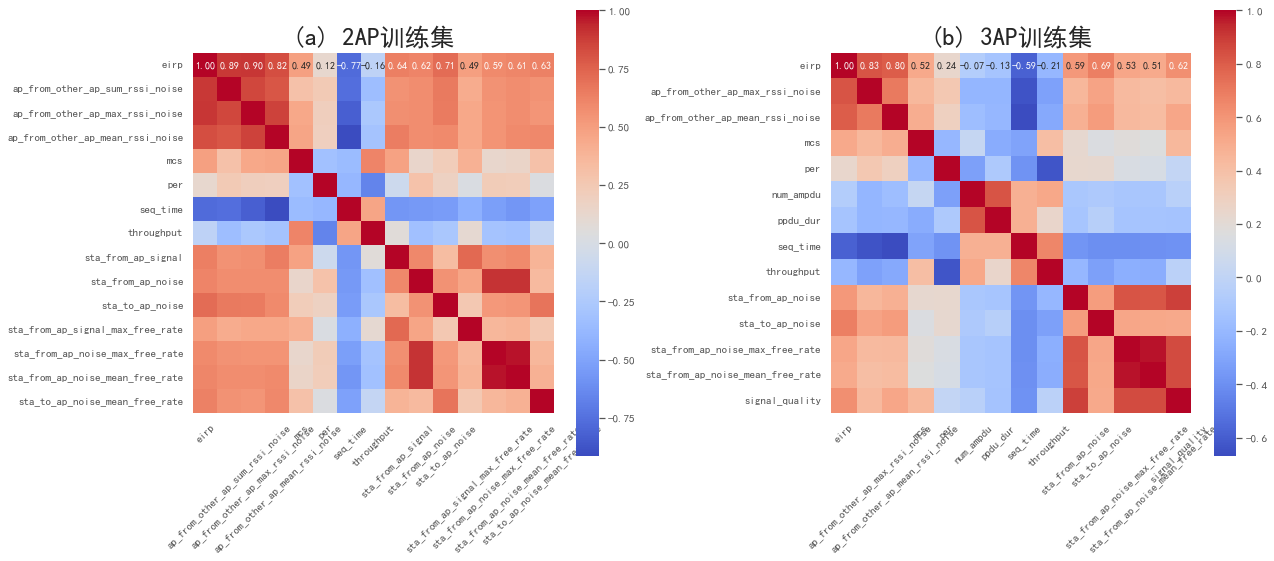
\includegraphics[width=1\linewidth]{figures/问题一热力图}
	\caption{参数相关性热力图}
	\label{fig:}
\end{figure}


如图所示,本节分析了在2AP和3AP训练集中,各参数与目标变量seq\_time之间的相关性。通过计算相关性,能够识别出对seq\_time影响显著的特征,并对其影响强弱进行排序。如表5.4所示。

\begin{longtable}{ccc}
	\caption{seq\_time影响强弱相关性(部分)}\\
	\hline
	\textbf{变量名} & \textbf{2AP} & \textbf{3AP} \\ 
	\hline
	throughput                          & 0.467841      & 0.660084      \\
	MCS                                & -0.353371     & -0.314458     \\
	per                                & -0.384524     & -0.385909     \\
	sta\_from\_ap\_signal\_max\_free\_rate & -0.430447     & -            \\
	sta\_to\_ap\_noise\_mean\_free\_rate & -0.513676     & -            \\
	sta\_from\_ap\_noise\_max\_free\_rate  & -0.528735     & -0.400428     \\
	sta\_to\_ap\_noise                    & -0.543609     & -0.404161     \\
	sta\_from\_ap\_noise                  & -0.558357     & -0.374620     \\
	sta\_from\_ap\_signal                 & -0.570747     & -            \\
	sta\_from\_ap\_noise\_mean\_free\_rate & -0.572061     & -0.396948     \\
	ap\_from\_other\_ap\_sum\_rssi\_noise & -0.761089     & -            \\
	eirp                               & -0.774949     & -0.585820     \\
	ap\_from\_other\_ap\_max\_rssi\_noise & -0.826892     & -0.634508     \\
	ap\_from\_other\_ap\_mean\_rssi\_noise & -0.912509     & -0.666785     \\ 
	\hline
\end{longtable}

1. 强影响因素:throughput在两类训练集下均为最高的正相关;多个变量(如 MCS、per 和 eirp)对seq\_time的影响均显著,表明了它们在预测seq\_time的重要性。

2. 负相关因素:eirp 和 RSSI 相关的变量均表现出较大的负相关;

3. 共性:在对2AP和3AP训练集的比较中,我们发现参数与seq\_time之间的关系呈现出一些共性,主要表现在以下几个方面:

\begin{itemize}
	\item 多数与RSSI相关的参数(如 ap\_from\_other\_ap\_mean\_rssi\_noise )在两个训练集中均表现出较高的负相关性。这表明信号的噪声和质量对发送数据帧序列的总时长(seq\_time)具有重要影响。
	\item 除RSSI相关参数外,eirp(AP的发送功率)在两个训练集中显示出显著的负相关性。
\end{itemize}


4.结论:尽管与RSSI相关的参数在影响seq\_time方面表现出一定的相关性,然而这些参数不足以支持训练高效的seq\_time预测模型,主要原因在于:

\begin{itemize}
	\item RSSI作为信号强度的度量,其值可能会受到环境干扰的极大影响,导致其对于模型学习的可预测性差。
	\item 相关性虽然显示出一定的影响,但并不能直接作为因果关系的依据。高相关性不一定意味着高因果解释力。
	\item 训练集中,与RSSI相关的参数多达20条及以上,数据维度过高可能导致过拟合及计算效率低下。
\end{itemize}

因此,有必要针对 RSSI 的相关参数进行进一步的提取和选择,并重新对RSSI进行特征构建,以提高预测模型的学习特征能力,通过计算和引入更具解释性的特征来增强模型的表达能力,将对模型的有效性和可预测性有积极影响。


\subsection{特征构建}


\subsubsection{信干噪比}

在传输过程中,信干燥比SINR可以代表着信号中所承载有效信息的比例,参考(4.1)



在公式中,由于训练集没有收集到信号或是干扰与噪声的功率大小,而RSSI一般以dBm(分贝毫瓦)表示,是接收端感知的信号强度。因此,实际上已经是信号功率的一个直接度量,所以本文在计算SINR时,由于RSSI是以功率的对数为基准的数量关系,故本文利用RSSI之间的差值来近似表示SINR。公式如下:


\begin{equation}
	RSSI_i-RSSI_j\lg \left( P_i \right) -\lg \left( P_j \right) =\lg \left( \frac{P_i}{P_j} \right) \frac{P_i}{P_j}
\end{equation}

由题可知,计算SINR的情况分为三种,故需要通过数据中AP与AP之间、AP与STA之间,STA与STA之间传输的RSSI数值大小来区分此次传输属于同步传输、异步传输还是混合传输。

\begin{table}[H]
	\centering
	\caption{不同传输形式下的RSSI监听情况}
	\begin{tabular}{@{}cccccc@{}} % 修改列数为6
		\toprule
		\textbf{类别序号} & \textbf{\shortstack{AP与AP \\ 监听RSSI}} & \textbf{\shortstack{关联AP与STA \\ 监听RSSI}} & \textbf{\shortstack{邻区AP与STA \\ 监听RSSI}} & \textbf{\shortstack{STA与STA \\ 监听RSSI}} & \textbf{传输形式} \\ \midrule
		1 & 较低 & 较高 & 较低 & 较低 & 同步传输 \\
		2 & 较低 & 较高 & 较高 & 较低 & 异步传输 \\
		3 & 时高时低 & 较高 & 时高时低 & 较低 & 混合传输 \\ \bottomrule
	\end{tabular}
\end{table}

然后通过判断不同的传输类型,可以进一步将公式(5.14)细化为:
 

\begin{equation}
	\left\{ 
	\begin{array}{l}
		\begin{matrix}
			SINR_{ST} \approx RSSI_{APtoSTA} - RSSI_N & \text{,} \text{同步传输} \\
		\end{matrix} \\[1ex]
		\begin{matrix}
			SINR_{AT} \approx RSSI_{APtoSTA} - RSSI_{neiborAPtoSTA} & \text{,} \text{异步传输} \\
		\end{matrix} \\[1ex]
		\begin{matrix}
			SINR_{MT} \approx \alpha \cdot SINR_{ST} + \left( 1 - \alpha \right) SINR_{AT} & \text{,} \text{混合传输} \\
		\end{matrix} \\
	\end{array} 
	\right.
\end{equation}


由此可以通过监听四类RSSI(sum列)来构建新的特征值SINR。

同时对于其他RSSI(max列和mean列)根据题中所提出的利用RSSI的最大值对CCA门限(PD门限与ED门限)做比较来判断数据在传输过程中是否能够正常发送并接收,利用RSSI的均值来与NAV门限做比较来判断是否要进行信道占用。所以利用这两列对不同要求门限的数值进行比较,算出其max列与mean列的信道通过率大小作为新特征值,其中CCA门限较为复杂,对于一个单元个中的数据列表中所有RSSI数值,如果小于PD门限则表示信号较弱,不能接收,若处于PD与ED门限之间,则认为它有$\beta_1$的概率携带PHY的preamble前导序列头,则端口识别为同频下的信号,这时候需要对PD门限进行比较,但他的RSSI处在PD和ED之间,则故有$\beta_1$的概率可以判断为信道繁忙,则代表信号不会收到新的数据传输干扰,同理在超过ED门限的RSSI中,有$\beta_2$的概率可以正确识别判断为信号传输判断信道繁忙,则也会成功通过信道传输。



\subsubsection{信号质量}



信号质量通常通过接收到的信号强度来衡量。因此,RSSI 值越高,表示信号质量越好。为了综合考虑来自不同 AP 的信号质量。本文对于STA端口,在收到AP的信号后,不论是两个AP的基本服务集还是三个AP的基本服务集,对STA收到的AP端口的信号进行加权平均处理,使用公式(4.7)计算得到一个综合的信号质量指标。




\subsection{模型建立与求解}

针对问题一,本文采用Stacking集成学习模型,将梯度提升学习算法,随机森林,支持向量回归以及线性回归四类算法结合起来。原因如下:

1.本题的训练集特征维度高,单一模型无法充分捕捉数据中的复杂关系。

2.训练集具有复杂性和多样性,单一模型无法有效捕捉所有的数据特征。

3.训练集样本有限,简单模型会导致高偏差,而复杂模型会造成过拟合。

4.Stacking的主要目的是提高模型的准确性和鲁棒性,特别适用于本题对准确性要求极高的场景


% TODO: \usepackage{graphicx} required
\begin{figure}[H]
	\centering
	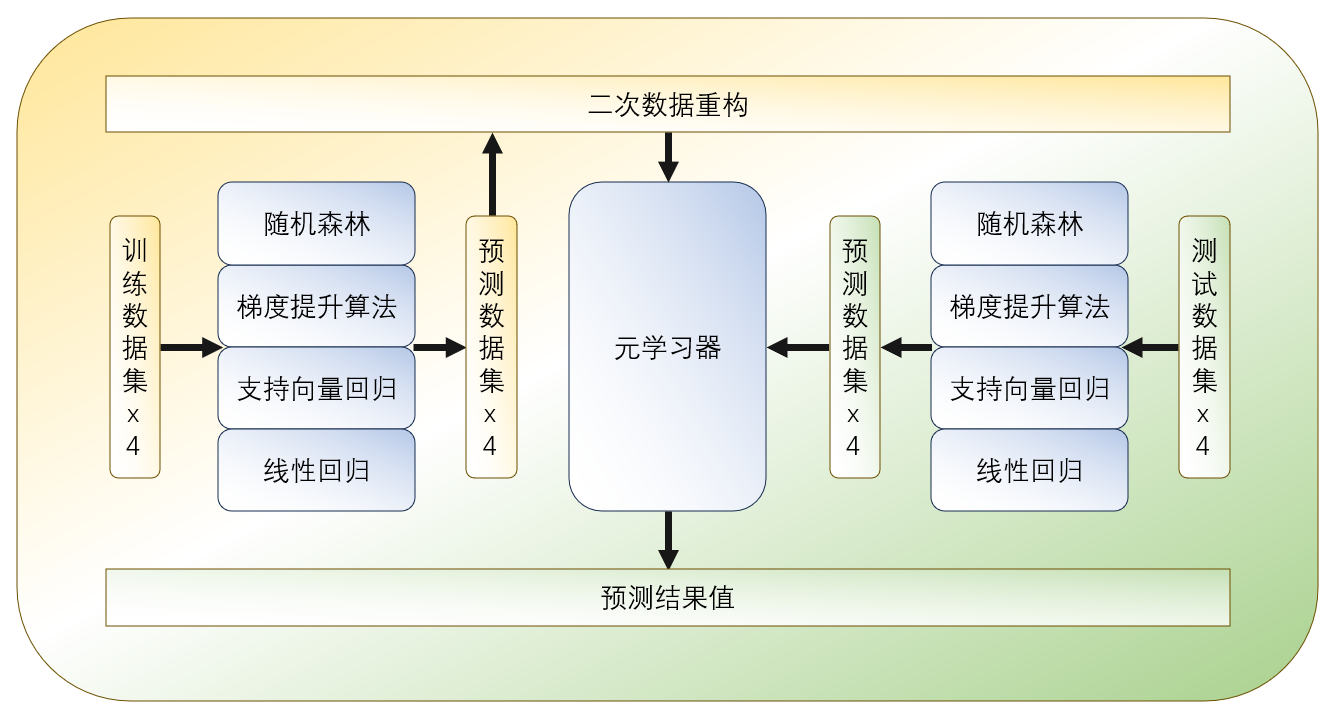
\includegraphics[width=0.7\linewidth]{figures/stacking}
	\caption{Stacking集成学习流程图}
	\label{fig:Stacking集成学习流程图}
\end{figure}

如图5.6所示,本文先将训练集放入多个基学习器中进行训练,将第一次预测的值以及训练集的目标值作为输入与输出进行数据的二测重构,放入元学习器中进行训练;测试集的特征值让四个基学习器中预测的值作为元学习器的输入值进行预测,得到的最终结果即为stacking集成学习最终的预测结果。训练使用的特征值如下表所示。

\begin{table}[H]
	\centering
	\caption{特征值(部分)}
	\begin{tabular}{ccccc} % 
		\toprule
		SINR & protocol & signal\_quality &  per & eirp\\ 
		\midrule
		 30.064 & 20 & -72.2375 &  0.27 & 13 \\
		 25 & 20 & -83.975 &  0.15 & 9 \\
	 	 25 & 8 & -83.975 &  0.14 & 9 \\
		 25.6628 & 20 & -83.8 &  0.17 & 10 \\
		\bottomrule
	\end{tabular}
\end{table}

使用Python的sklearn库,构建集成学习模型,将数据集按照7:3的比例划分为训练集和测试集,然后使用网格搜索进行超参数优化,以找到性能最佳的模型参数组合,训练出最优模型,结果如下。


\begin{table}[H]
	\centering
	\caption{模型性能对比}
	\begin{tabular}{@{}ccccccc@{}}
		\toprule
		\multirow{2}{*}{Model} & \multicolumn{2}{c}{2AP} & \multicolumn{2}{c}{3AP} & \multicolumn{2}{c}{AP} \\ 
		\cmidrule{2-3}
		\cmidrule{4-5}
		\cmidrule{6-7}
		& RMSE & R² & RMSE & R² & RMSE & R² \\ 
		\midrule
		梯度提升 & 2.747696 & 0.932200 & 3.269128 & 0.926637 & 7.125881 & 0.682336 \\
		随机森林 & 2.672078 & 0.935880 & 3.216168 & 0.928995 & 6.781550 & 0.712294 \\
		支持向量回归 & 3.589683 & 0.884281 & 4.743004 & 0.845575 & 8.301113 & 0.568914 \\
		线性回归 & 3.099190 & 0.913744 & 4.347454 & 0.870258 & 9.004967 & 0.492711 \\
		集成学习 & 2.606650 & 0.938982 & 3.102912 & 0.933908 & 6.746497 & 0.715260 \\
		集成学习(优化参数) & 1.453308 & 0.981033 & 2.757210 & 0.947814 & 6.615275 & 0.726229 \\ 
		\bottomrule
	\end{tabular}
\end{table}










如表5.7所示,本文对AP个数进行分类建模(2AP和3AP),分别训练模型,同时对AP数量统一建模,以比较集成学习模型在不同样本下的模型性能。显然,对AP数量分类后,预测性能最优。经过5重交叉验证和网格搜索调参后,最优的参数组合如下表所示。

\begin{table}[H]
	\centering
	\caption{最佳得分和参数设置}
	\begin{tabular}{cc}
		\toprule
		指标 & 最佳值 \\
		\midrule
		最佳得分 (Best Score) & 9.77534051567329 \\
		学习率 (learning\_rate) & 0.3 \\
		基学习器数量 (n\_estimators) - 梯度提升 & 200 \\
		最大深度 (max\_depth) - 随机森林 & 5 \\
		基学习器数量 (n\_estimators) - 随机森林 & 200 \\
		惩罚参数 (C) - 支持向量回归 & 10 \\
		核函数 (kernel) - 支持向量回归 & `rbf' \\
		\bottomrule
	\end{tabular}
\end{table}





% TODO: \usepackage{graphicx} required
\begin{figure}[H]
	\centering
	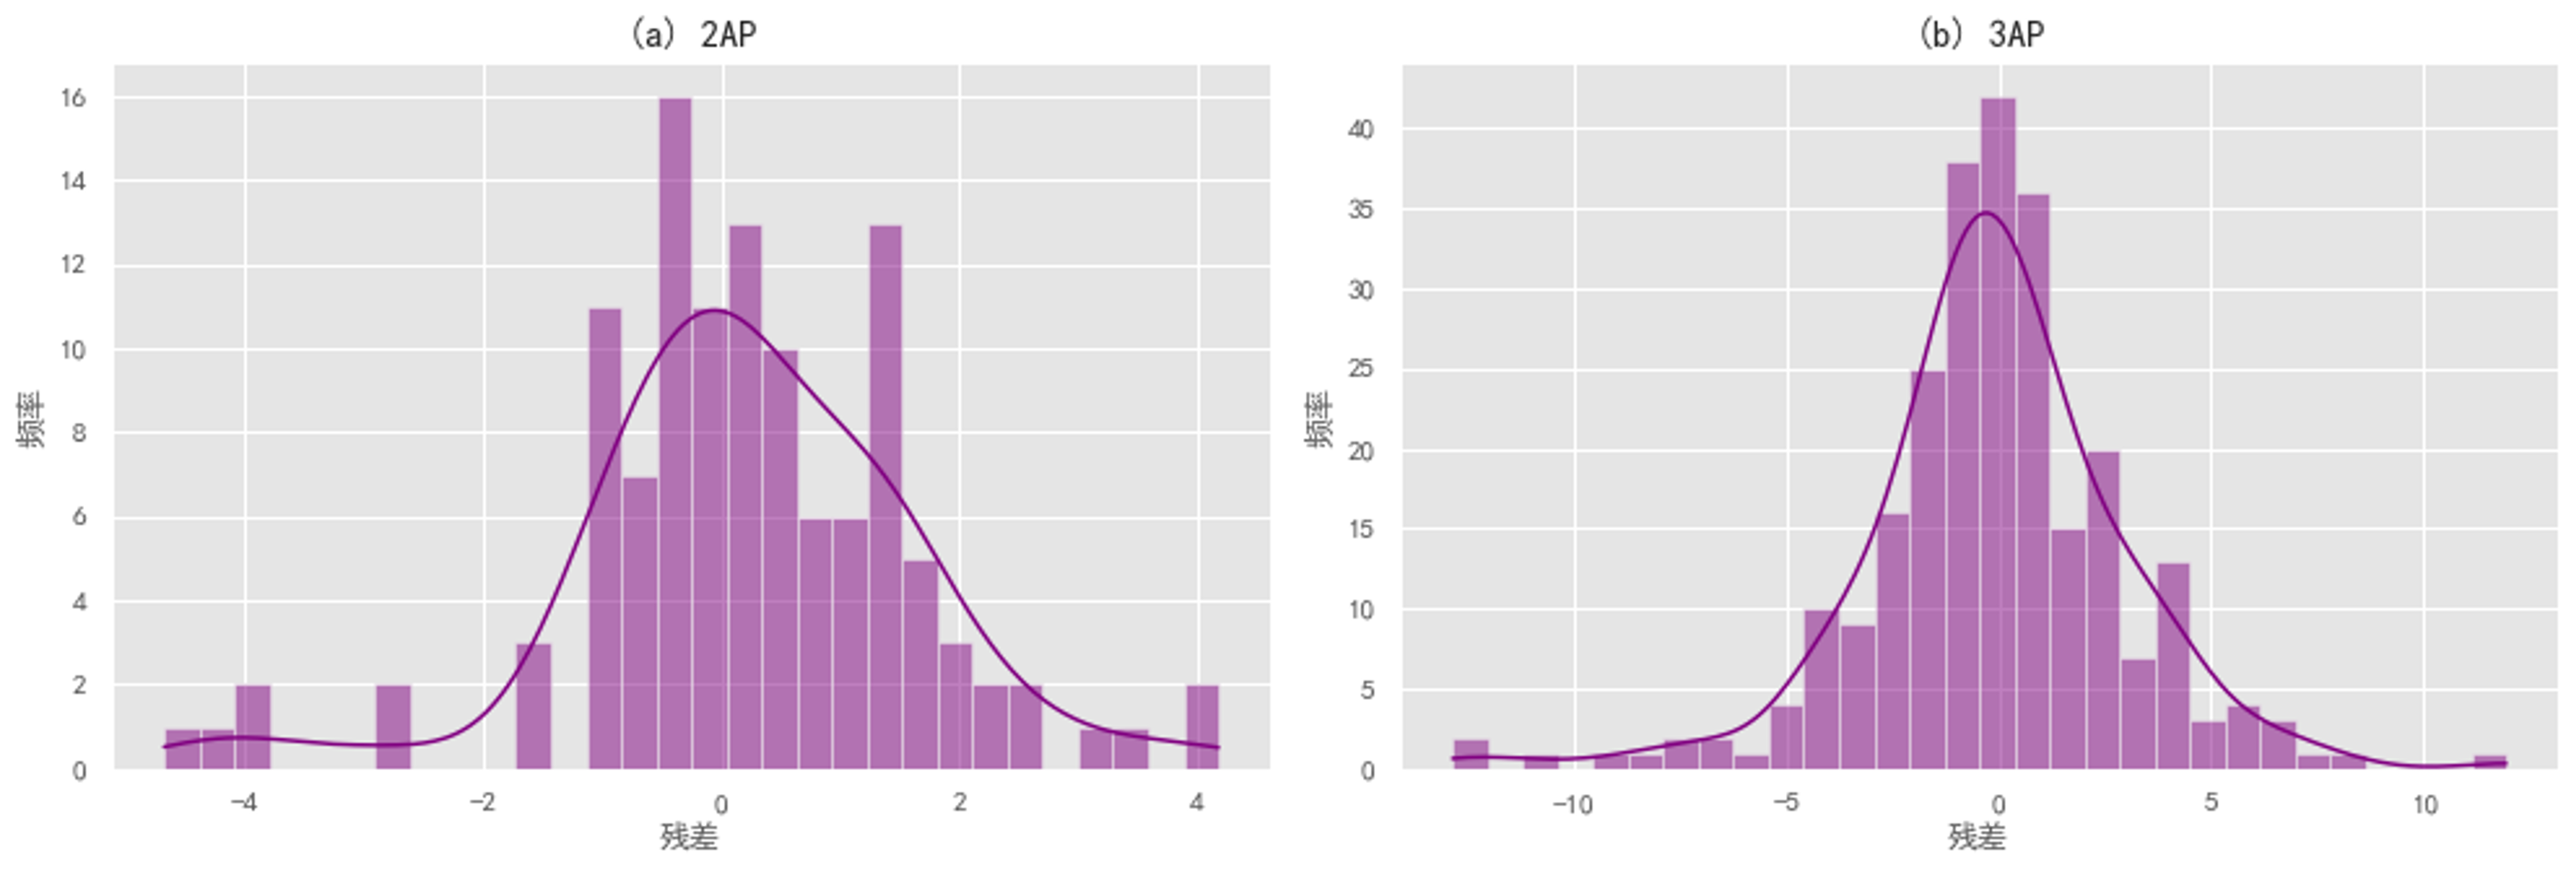
\includegraphics[width=0.9\linewidth]{figures/2ap和3ap残差图}
	\caption{Stacking模型残差分布图}
	\label{fig:2ap3ap}
\end{figure}


% TODO: \usepackage{graphicx} required
\begin{figure}[H]
	\centering
	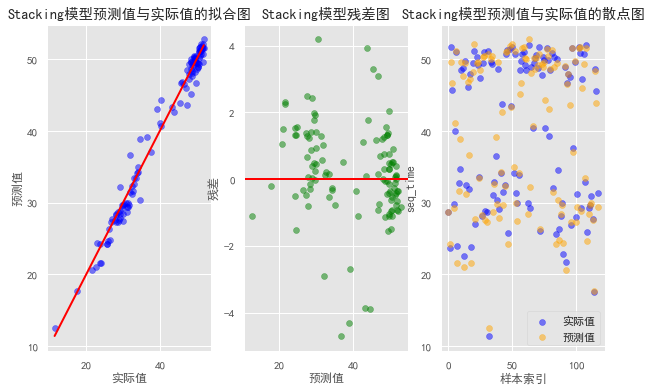
\includegraphics[width=0.8\linewidth]{figures/2ap结果}
	\caption{Stacking模型预测图}
	\label{fig:2ap}
\end{figure}



如图所示,对于2AP预测模型,残差主要分布在[ -2,+2 ]之间,测试集的平均绝对误差(MSE)为1.05,决定系数${R}^{2}$为0.98,模型预测精度较高;对于3AP预测模型,残差主要分布在[ -5,+5 ]之间,测试集的平均绝对误差(MSE)为1.84,决定系数${R}^{2}$为0.95,模型预测精度也较高,可以实现对seq\_time的高精度预测。



\section{问题二分析与求解}
\subsection{问题二分析}
针对问题二,我们将在有效显著特征的基础上,对(MCS, NSS)组合进行模型训练与预测。与问题一的主要区别在于,此次预测的是一组相互独立的数组对。根据分析,数据传输的质量在一定程度上影响了 MCS 的取值。信干噪比(SINR)作为反映传输数据质量的关键特征,当 SINR 较大时,表明信号相对于干扰与噪声非常明显,这意味着该组信号属于高质量信号。在这种情况下,传输信号所需的 MCS 取值通常较高。

对于 NSS 的选择,它在一定程度上依赖于传输设备的硬件配置。在数据中,NSS 有两个取值:1 和 2。不同的 NSS 值对应着 12 种 MCS 值,形成 24 种不同的 PHYRate 组合,见表4.3。这些因素共同作用,为模型的训练与预测提供了基础。



对此构建模型,用来预测MCS与NSS的值大小,可以直接对MCS和NSS进行预测,也可以通过预测PHY Rate来反向推导出MCS与NSS 的大小。但是查看表格可以看到(MCS,NSS)与PHY Rate之间只存在单向映射关系,即MCS和NSS组合可以得到PHY Rate,但是PHY Rate并不一定可以反推得到MCS和NSS组合如[MCS,NSS]为[5,1]和[3,2]下的PHYRate同为68.8。这不是本题想要看到的结果。所以本文选择对MCS和NSS进行直接预测。


% TODO: \usepackage{graphicx} required
\begin{figure}[H]
	\centering
	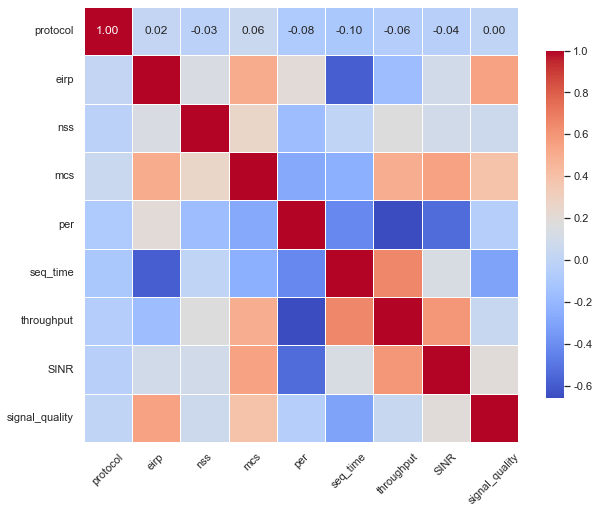
\includegraphics[width=0.7\linewidth]{figures/问题2热力图}
	\caption{(MCS,NSS)与各变量相关性热力图}
	\label{fig:2}
\end{figure}


如图6.8所示,首先,结合实测训练集中的测试基本信息和问题一的特征构建,分别对MCS和NSS进行相关性分析,初步寻找特征值。显然,各变量与MCS的相关性显著更强,有5个变量的相关性在0.5以上,其中,MCS与SINR和信号质量两个变量的相关性最高;而各变量与NSS的相关性明显更弱,只与MCS有0.3的相关性,与其它变量相关性的绝对值位于0.1-0.2之间。


因此,本题考虑构建层次预测模型(Hierarchical Prediction Model),在这个模型中,首先通过高相关性的特征预测目标变量(MCS),然后将预测结果作为输入特征,进一步预测下一个目标变量(NSS)。这种方法的优势在于利用前一步骤中获得的信息,提高后续预测的准确性和可靠性。通过这种层次结构,可以更有效地捕捉变量间的复杂关系,从而实现更优的预测效果。



\subsection{上层预测模型的建立与求解}

根据上述分析,本节利用相关特征值先做上层预测模型的建立。首先,将给定的数据进行训练集与测试集的划分,利用上述相关特征对分类变量MCS预测,考虑到问题一中的Stacking集成学习方法,继续将梯度提升方法、随机森林、支持向量机分类、线性分类进行集成学习,训练后的最优参数如下表所示。

\begin{table}[H]
	\centering
	\caption{最佳得分和参数设置}
	\begin{tabular}{cc}
		\toprule
		指标 & 最佳值/参数设置 \\
		\midrule
		最佳得分 (Best Score) & 0.7223124480220936 \\
		学习率 (Learning Rate) - 梯度提升 & 0.1 \\
		基学习器数量 (N\_estimators) - 梯度提升 & 200 \\
		最大特征 (Max Features) - 随机森林 & `sqrt' \\
		基学习器数量 (N\_estimators) - 随机森林 & 200 \\
		惩罚参数 (C) - 支持向量分类器 & 10 \\
		惩罚类型 (Penalty) - 最终估计器 & `l2' \\
		惩罚参数 (C) - 最终估计器 & 1 \\
		\bottomrule
	\end{tabular}
\end{table}


\begin{table}[H]
	\centering
	\caption{优化后的上层Stacking模型性能}
	\begin{tabular}{lcccc}
		\toprule
		& Accuracy & F1 Score & Precision & Recall \\
		\midrule
		& 0.8053333333333333 & 0.7972823937456768 & 0.7940897041448882 & 0.8053333333333333 \\
		\bottomrule
	\end{tabular}
\end{table}


% TODO: \usepackage{graphicx} required
\begin{figure}[H]
	\centering
	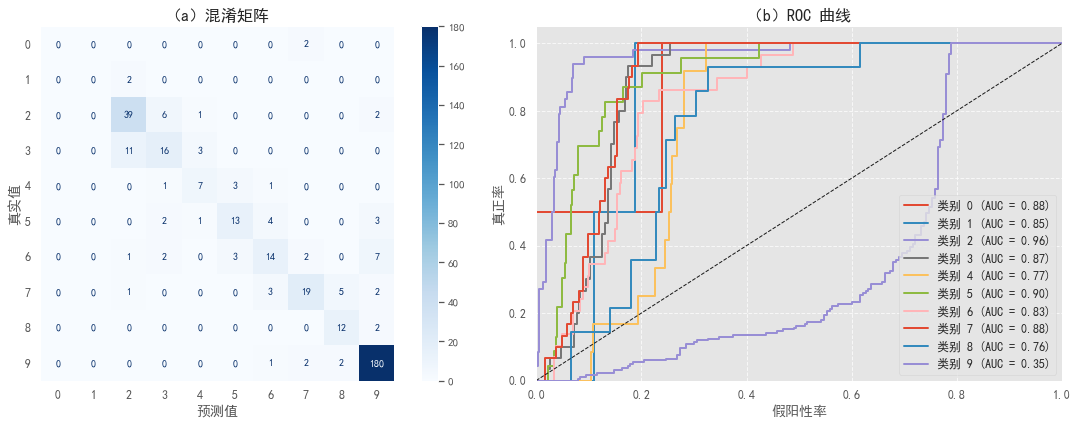
\includegraphics[width=1\linewidth]{figures/问题21预测结果图}
	\caption{分类性能评估图}
	\label{fig:21}
\end{figure}

如表6.10和图6.10所示,模型具有较高的准确率 (0.81),在整体上能够正确分类大部分样本,表现出良好的总体性能;F1 分数为0.80,表明模型在处理类别不平衡问题时,表现较为均衡;同时,具有高召回率 (0.81),模型能有效识别出大多数正类样本,降低假阴性的风险。尤其是在MCS训练集中,MCS的值共有12类,值是11的占比为48.32\%。

% TODO: \usepackage{graphicx} required
\begin{figure}[H]
	\centering
	\includegraphics[width=1\linewidth]{"figures/问题22预测结果png (2)"}
	\caption{测试集上的分类效果图}
	\label{fig:22png-2}
\end{figure}


如图6.11所示,尽管精确率尚未达到理想水平,且在其他类别的表现上仍有改进的空间,测试集上的分类效果图显示出模型预测的数量分布相对均匀。这表明,模型在处理不同类别时能够有效区分,未受到值为 11的类的干扰,反而正确地学习到了特征。

这样的结果不仅展示了模型对特定类别的良好适应性,也反映出其在特征提取和分类上的潜力,为进一步建立NSS下层预测模型奠定了基础。



\subsection{下层预测模型的建立与求解}

在 MCS上层预测模型的基础上,本节将 MCS 的预测值作为特征输入,构建对 NSS的 下层预测模型。然而。初步分析发现,NSS 的取值仅为 1 和 2,是二分类变量,且为1的数量比例极低,绝大部分 NSS类别为 2的占比为97.91\%。


在这种情况下,NSS 存在长尾分布特征,表明大多数样本集中在类别 2,而类别 1 的样本则非常稀少。如果仅依赖现有特征来建立模型进行分类预测,会导致模型过拟合,尤其是对高频类别的过度依赖,进而导致预测结果几乎全部为 2,无法有效捕捉到类别 1 的特征。


% TODO: \usepackage{graphicx} required
\begin{figure}[H]
	\centering
	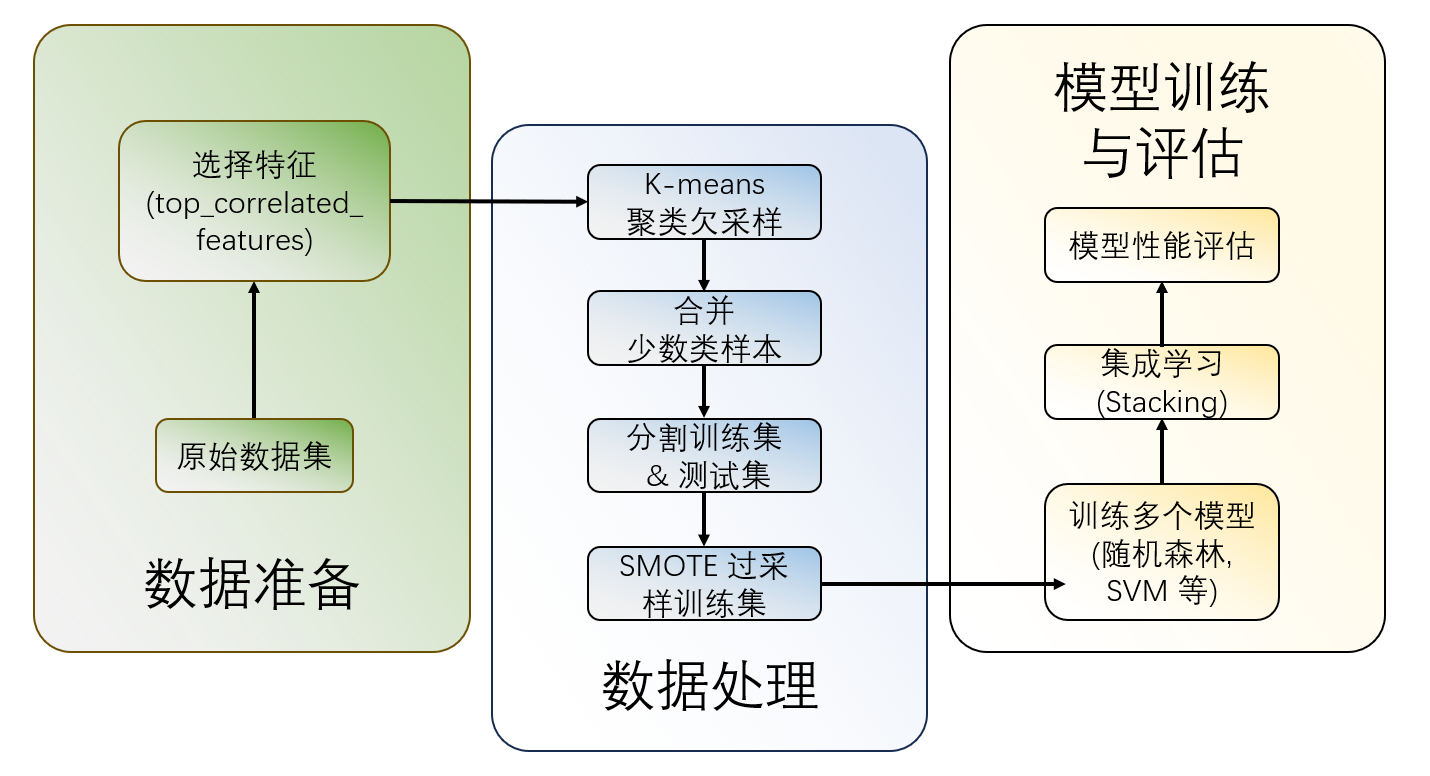
\includegraphics[width=0.7\linewidth]{figures/问题2采样流程}
	\caption{采样流程图}
	\label{fig:2}
\end{figure}

如图6.12所示,为了应对这一问题,本文使用了Kmeans聚类欠采样和SMOTE(合成少数类过采样技术)两种采样方法,以应对NSS的长尾分布特征。首先选择NSS值为2的多数类样本,使用K-means对多数类样本进行聚类,聚类簇数为11,然后从每个聚类中选择最有代表性的5个样本,最后合并代表性样本与少数类样本。

训练后的模型最佳参数如下表。

\begin{table}[H]
	\centering
	\caption{最佳得分和参数设置}
	\begin{tabular}{cc}
		\toprule
		指标 & 最佳值/参数设置 \\
		\midrule
		最佳得分 (Best Score) & 0.8421 \\
		学习率 (Learning Rate) - 梯度提升 & 0.01 \\
		基学习器数量 (N\_estimators) - 梯度提升 & 100 \\
		最大特征 (Max Features) - 随机森林 & `sqrt' \\
		基学习器数量 (N\_estimators) - 随机森林 & 100 \\
		惩罚参数 (C) - 支持向量分类器 & 10 \\
		惩罚类型 (Penalty) - 最终估计器 & `l2' \\
		惩罚参数 (C) - 最终估计器 & 1 \\
		\bottomrule
	\end{tabular}
\end{table}


\begin{table}[H]
	\centering
	\caption{优化后的下层Stacking模型性能}
	\begin{tabular}{lcccc}
		\toprule
		& Accuracy & F1 Score & Precision & Recall \\
		\midrule
		& 0.92 & 0.9226 & 0.9378 & 0.92 \\
		\bottomrule
	\end{tabular}
\end{table}

如表6.11和图6.13所示,F1 Score为0.9226,表明模型在处理NSS的不平衡样本时的性能较好,尤其在预测正类时表现出色。精确率高(0.9378),表明误报率较低。召回率同样较高(0.92),说明模型能够有效地识别正类和负类样本,未漏掉太多真实负类。


% TODO: \usepackage{graphicx} required
\begin{figure}[H]
	\centering
	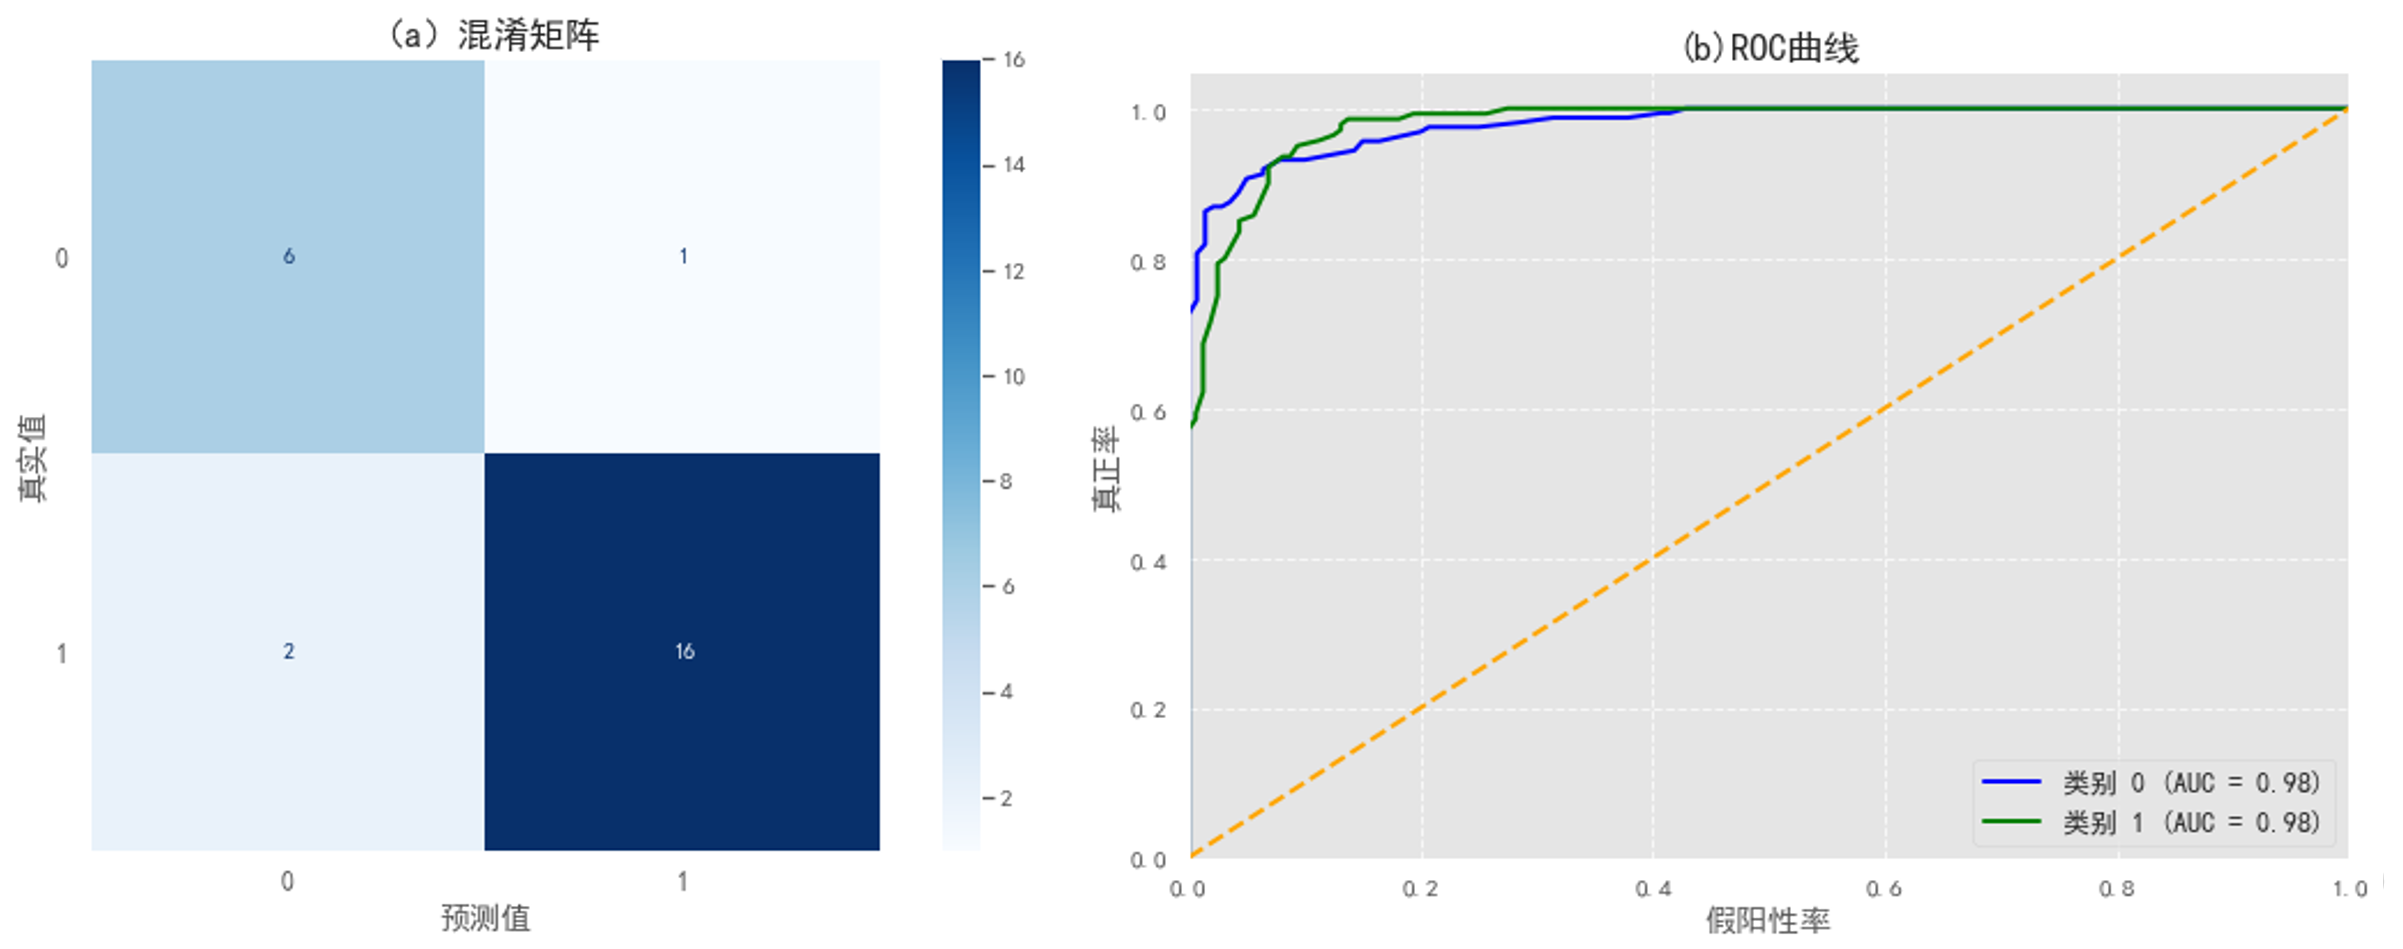
\includegraphics[width=1\linewidth]{figures/问题24}
	\caption{分类性能评估图}
	\label{fig:24}
\end{figure}


% TODO: \usepackage{graphicx} required
\begin{figure}[H]
	\centering
	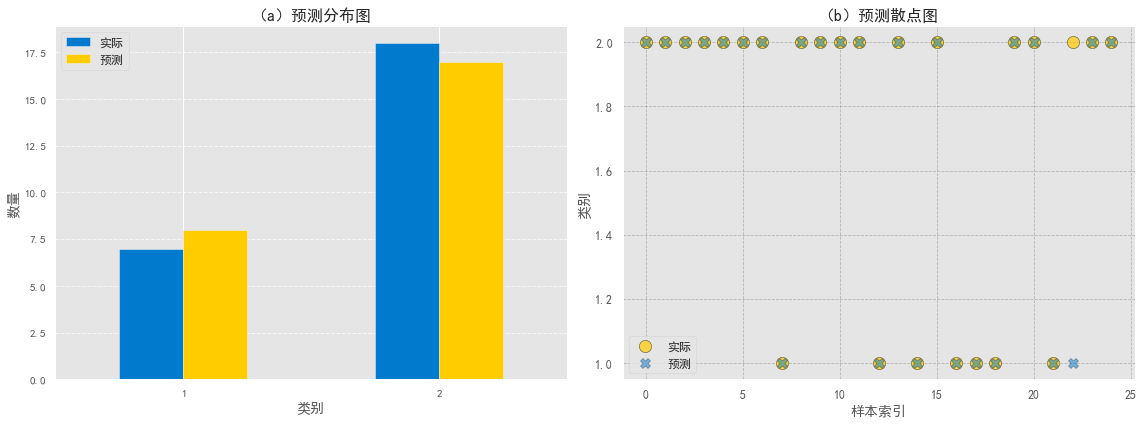
\includegraphics[width=1\linewidth]{figures/问题25}
	\caption{测试集上的分类效果图}
	\label{fig:23}
\end{figure}

根据图6.14,根据预测分布图和散点图的分析,可以看出下层预测模型对NSS的分类效果良好。散点图展示了正负样本在特征空间中的分布,模型成功地将不同NSS类别的样本分开,显示出良好的区分能力。此外,预测分布图表明模型有效解决了正负样本之间的极度不平衡问题,能够识别出各类别的特征值,增强了分类的可靠性和准确性。这表明模型在特征提取和样本分类方面的能力得到了显著提升。









\section{问题三分析与求解}
\subsection{问题三分析}
\subsubsection{随机回退机制分析}

问题三是建立在问题一和问题二的基础上,题中提到对于MCS与NSS的对应取值可以参考在数据中实际测到的数据数值对,加上其他的特征值对AP的吞吐量进行模型的训练与预测。同时通过第四章模型准备中的流程分析,可以得知在数据发送过程中会发生一定的AP冲突,这会导致双方AP的回退时间增加,同时本是经过一定随即回退时间后要完成数据的传输,现在反而浪费了时间却没有增加AP的吞吐量,所以退回时间在一定程度上直接影响着AP的吞吐量,以及系统的吞吐量。

在过程中可以知道每一次回退时间的期望值为$\frac{(CW-1)\times slotTime}{2}$,则其如果发生数据传输冲突,则会对CW进行翻倍,这时候他的时间窗口为$\left[ 0,CW\times 2-1\right] $,那么这时候为第二次回退期望时间为$\frac{(CW\times 2-1)\times slotTime}{2}$,故第n次回退时间的期望是$\frac{(CW\times 2^{n-1}-1)\times slotTime}{2}$。但是当$CW$翻倍到$CW_{max}$的时候$CW$将不会变动,直到成功接收到$ACK$才会将$CW$进行重置,则需要计算其最小值$\frac{1}{2}min(CW\times 2^{n-1}-1,CW_{max}-1)\times slotTime$。

但是上述是对第n次回退时的回退时间期望的求解,而如果要从系统的角度看,需要去计算第n次回退时累计回退期望时长,即

\begin{equation}\label{eq1}
	backoffTime=\frac{1}{2}\sum_{i=1}^{n} min(CW\times 2^{i-1}-1,CW_{max}-1)\times slotTime
\end{equation}


\begin{figure}[htbp]
	\centering
	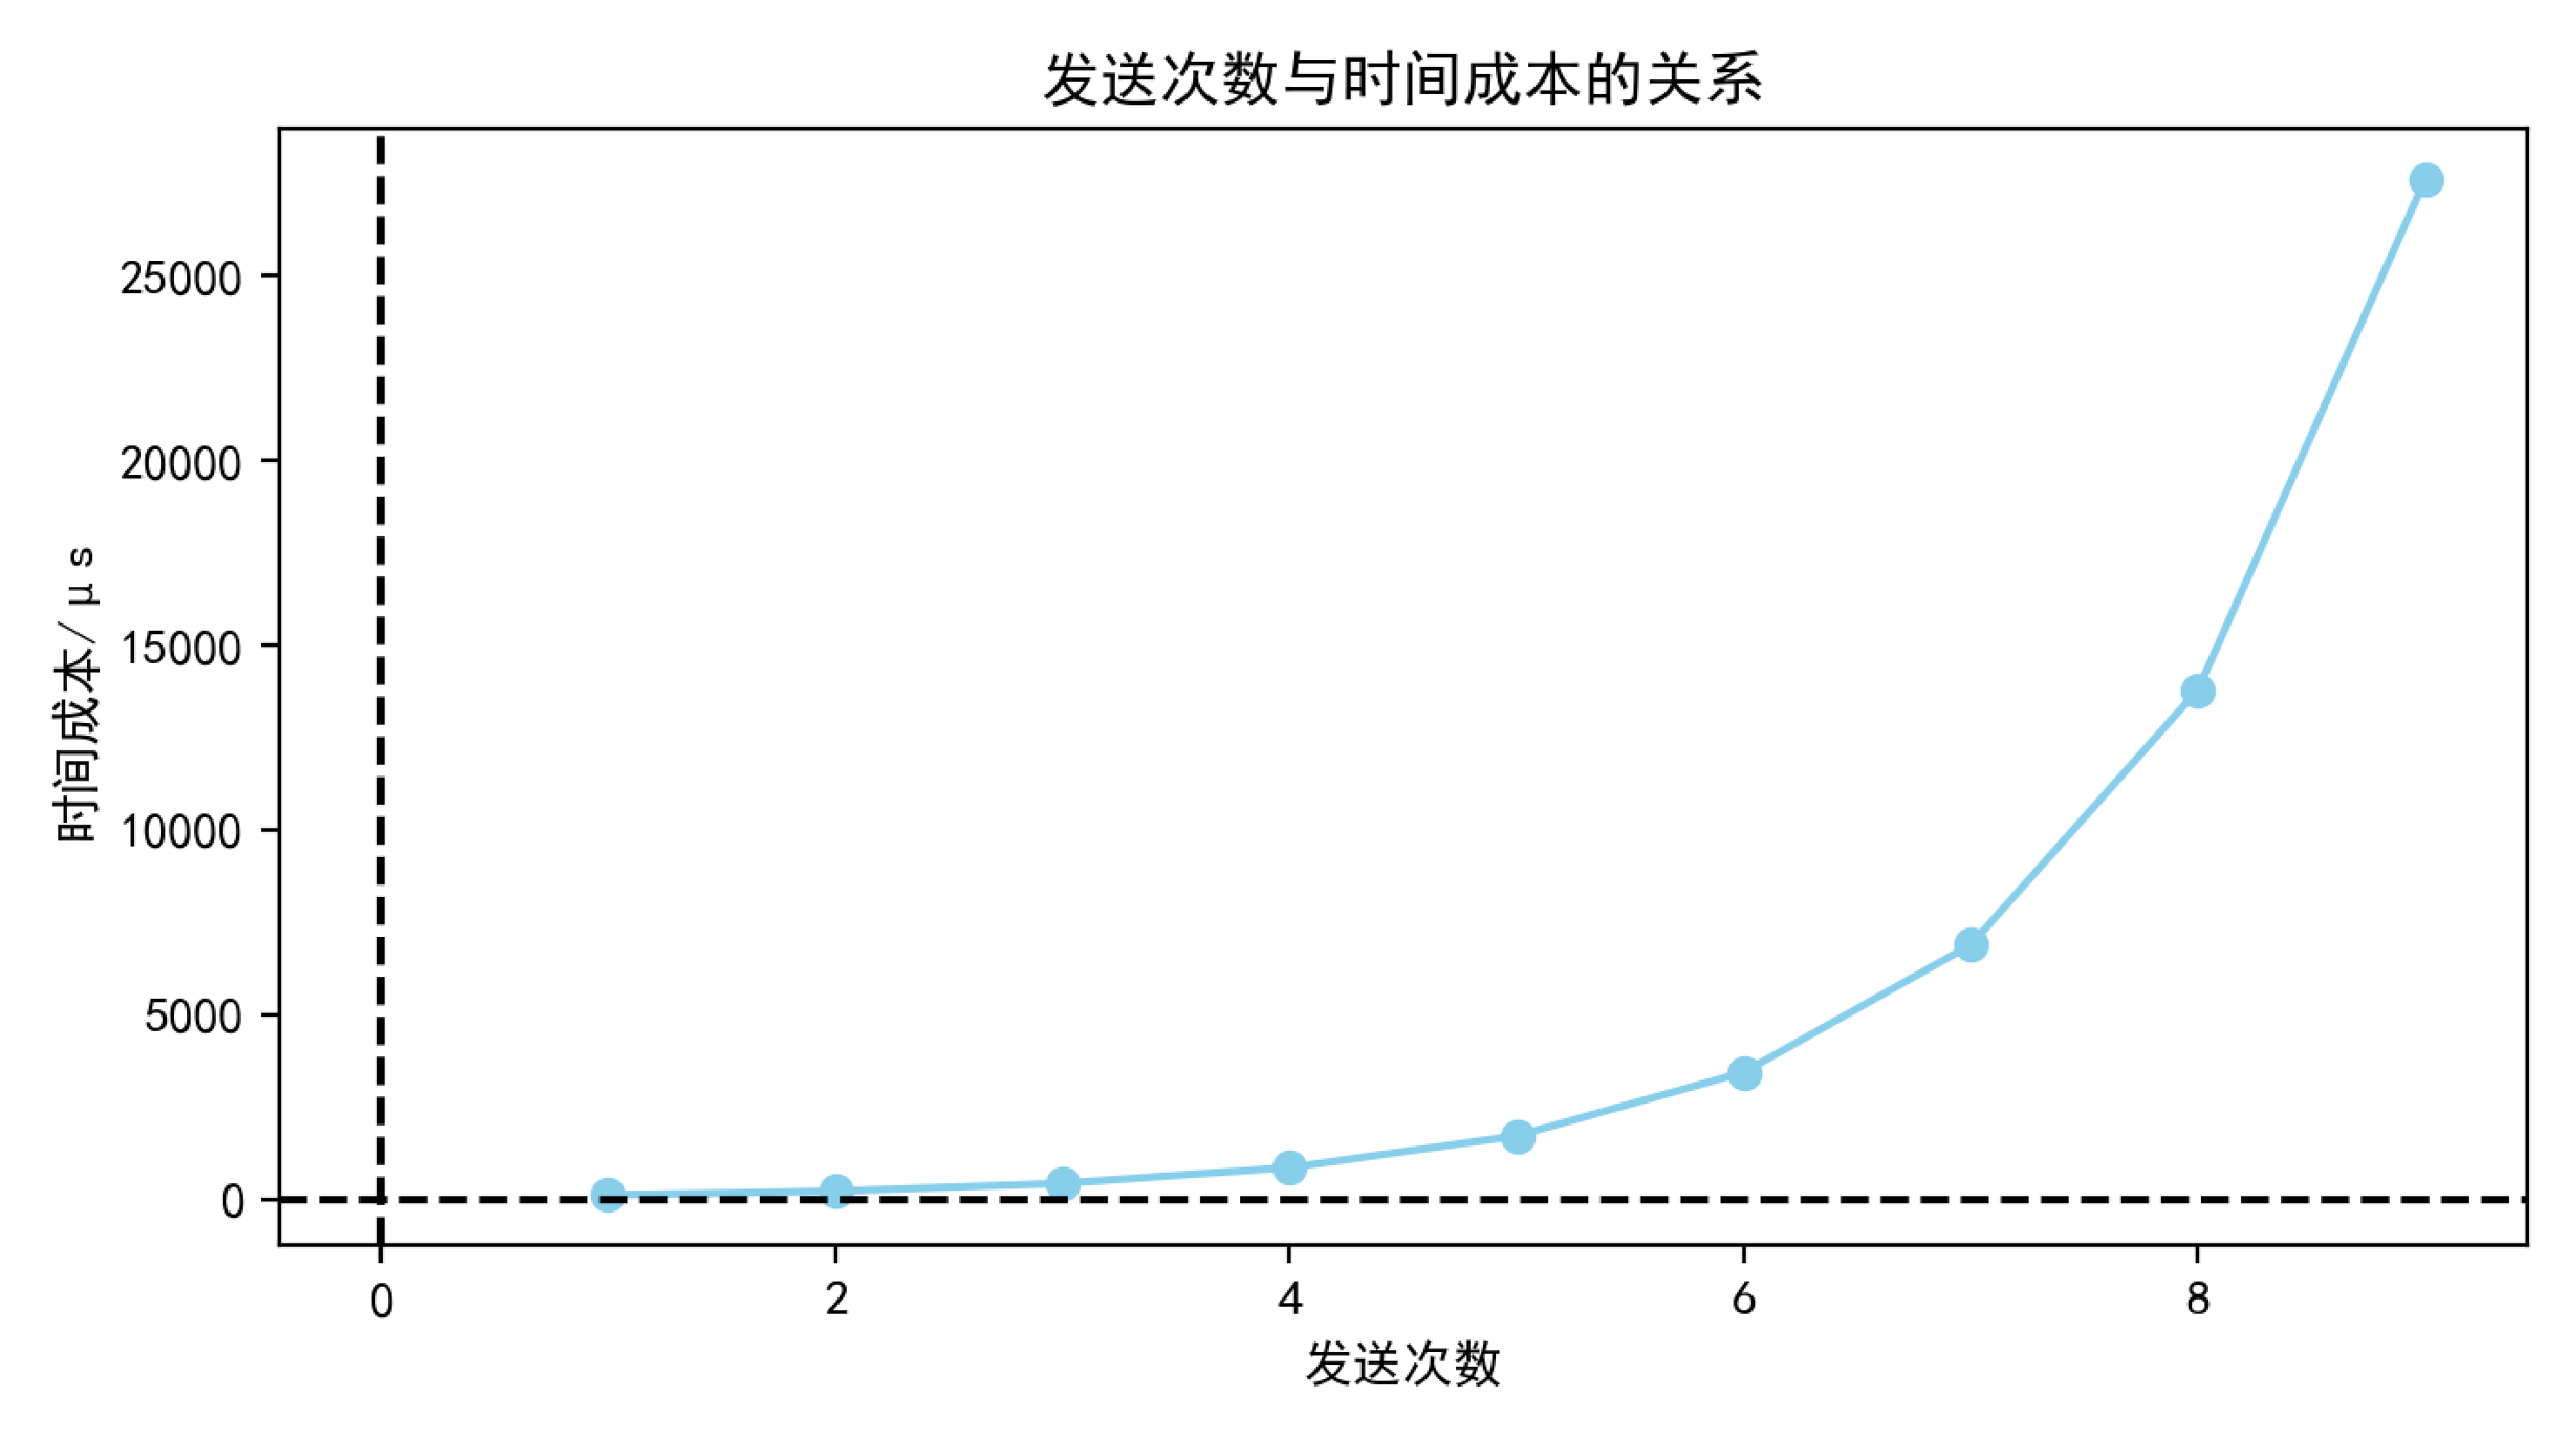
\includegraphics[width=0.75\linewidth]{2.eps}
	\caption{发送次数与时间成本折现图($ap\_num=2,CW_{min}=6,CW_{max}=2100$)}
	\label{figure2}
\end{figure}

同时第一次传输时随即回退时间窗格数量为$\frac{CW-1}{2}$,那么另一个AP在本AP随机回退的窗格数量中每一个停止的概率是相同的,所以另一个AP与本AP发生冲突的概率是$\frac{2}{CW-1}$,则等环境中一共有$ap\_Num$个AP时,他的冲突概率是$\frac{2(ap\_Num-1)}{CW-1}$,则其第n次不发生冲突的概率为

\begin{equation}
	P_{n}=1-\frac{2(ap\_Num-1)}{CW\times 2^{n-1}-1}
\end{equation}

\begin{figure}[H]
	\centering
	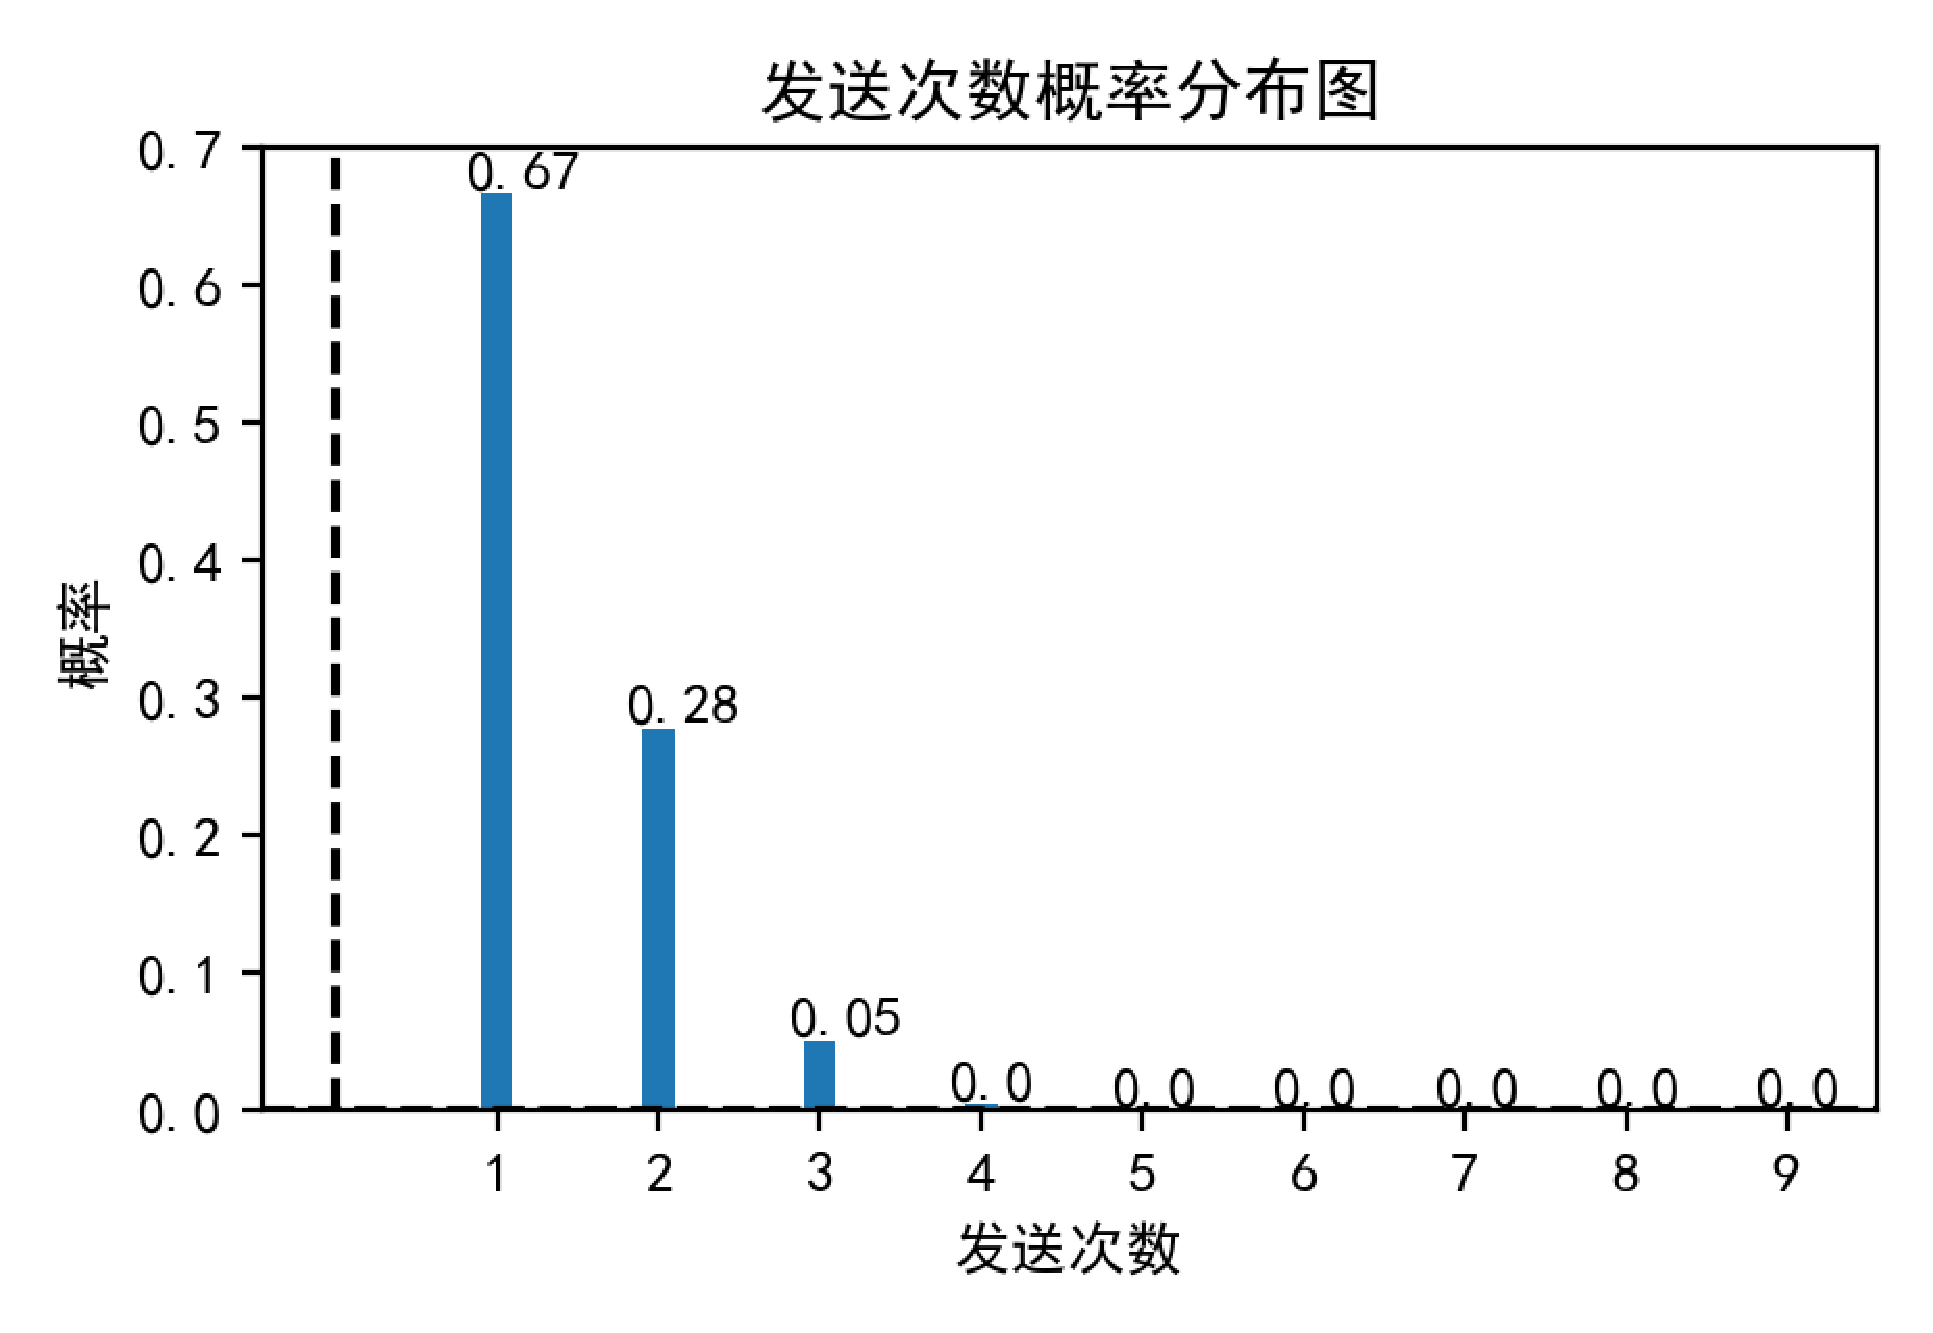
\includegraphics[width=0.75\linewidth]{1.eps}
	\caption{发送次数概率分布图($ap\_num=2,CW_{min}=6,CW_{max}=2100$)}
	\label{figure1}
\end{figure}


故当发生到第n次才能成功发送的概率服从以下分布:

\begin{equation}
	Pr_{(x=n)}=\prod_{i=1}^{n-1}{\left( 1-P_i \right) \times}P_n
\end{equation}

则可以利用$backoffTime$和$P_n$计算得到第n次期望的退回时间即新特征指标$BackMean$:

\begin{equation}
	BackMean=\sum_{i=1}^n{Pr_{(x=n)}\times backoffTime_i}
\end{equation}

\begin{figure}[H]
	\centering
	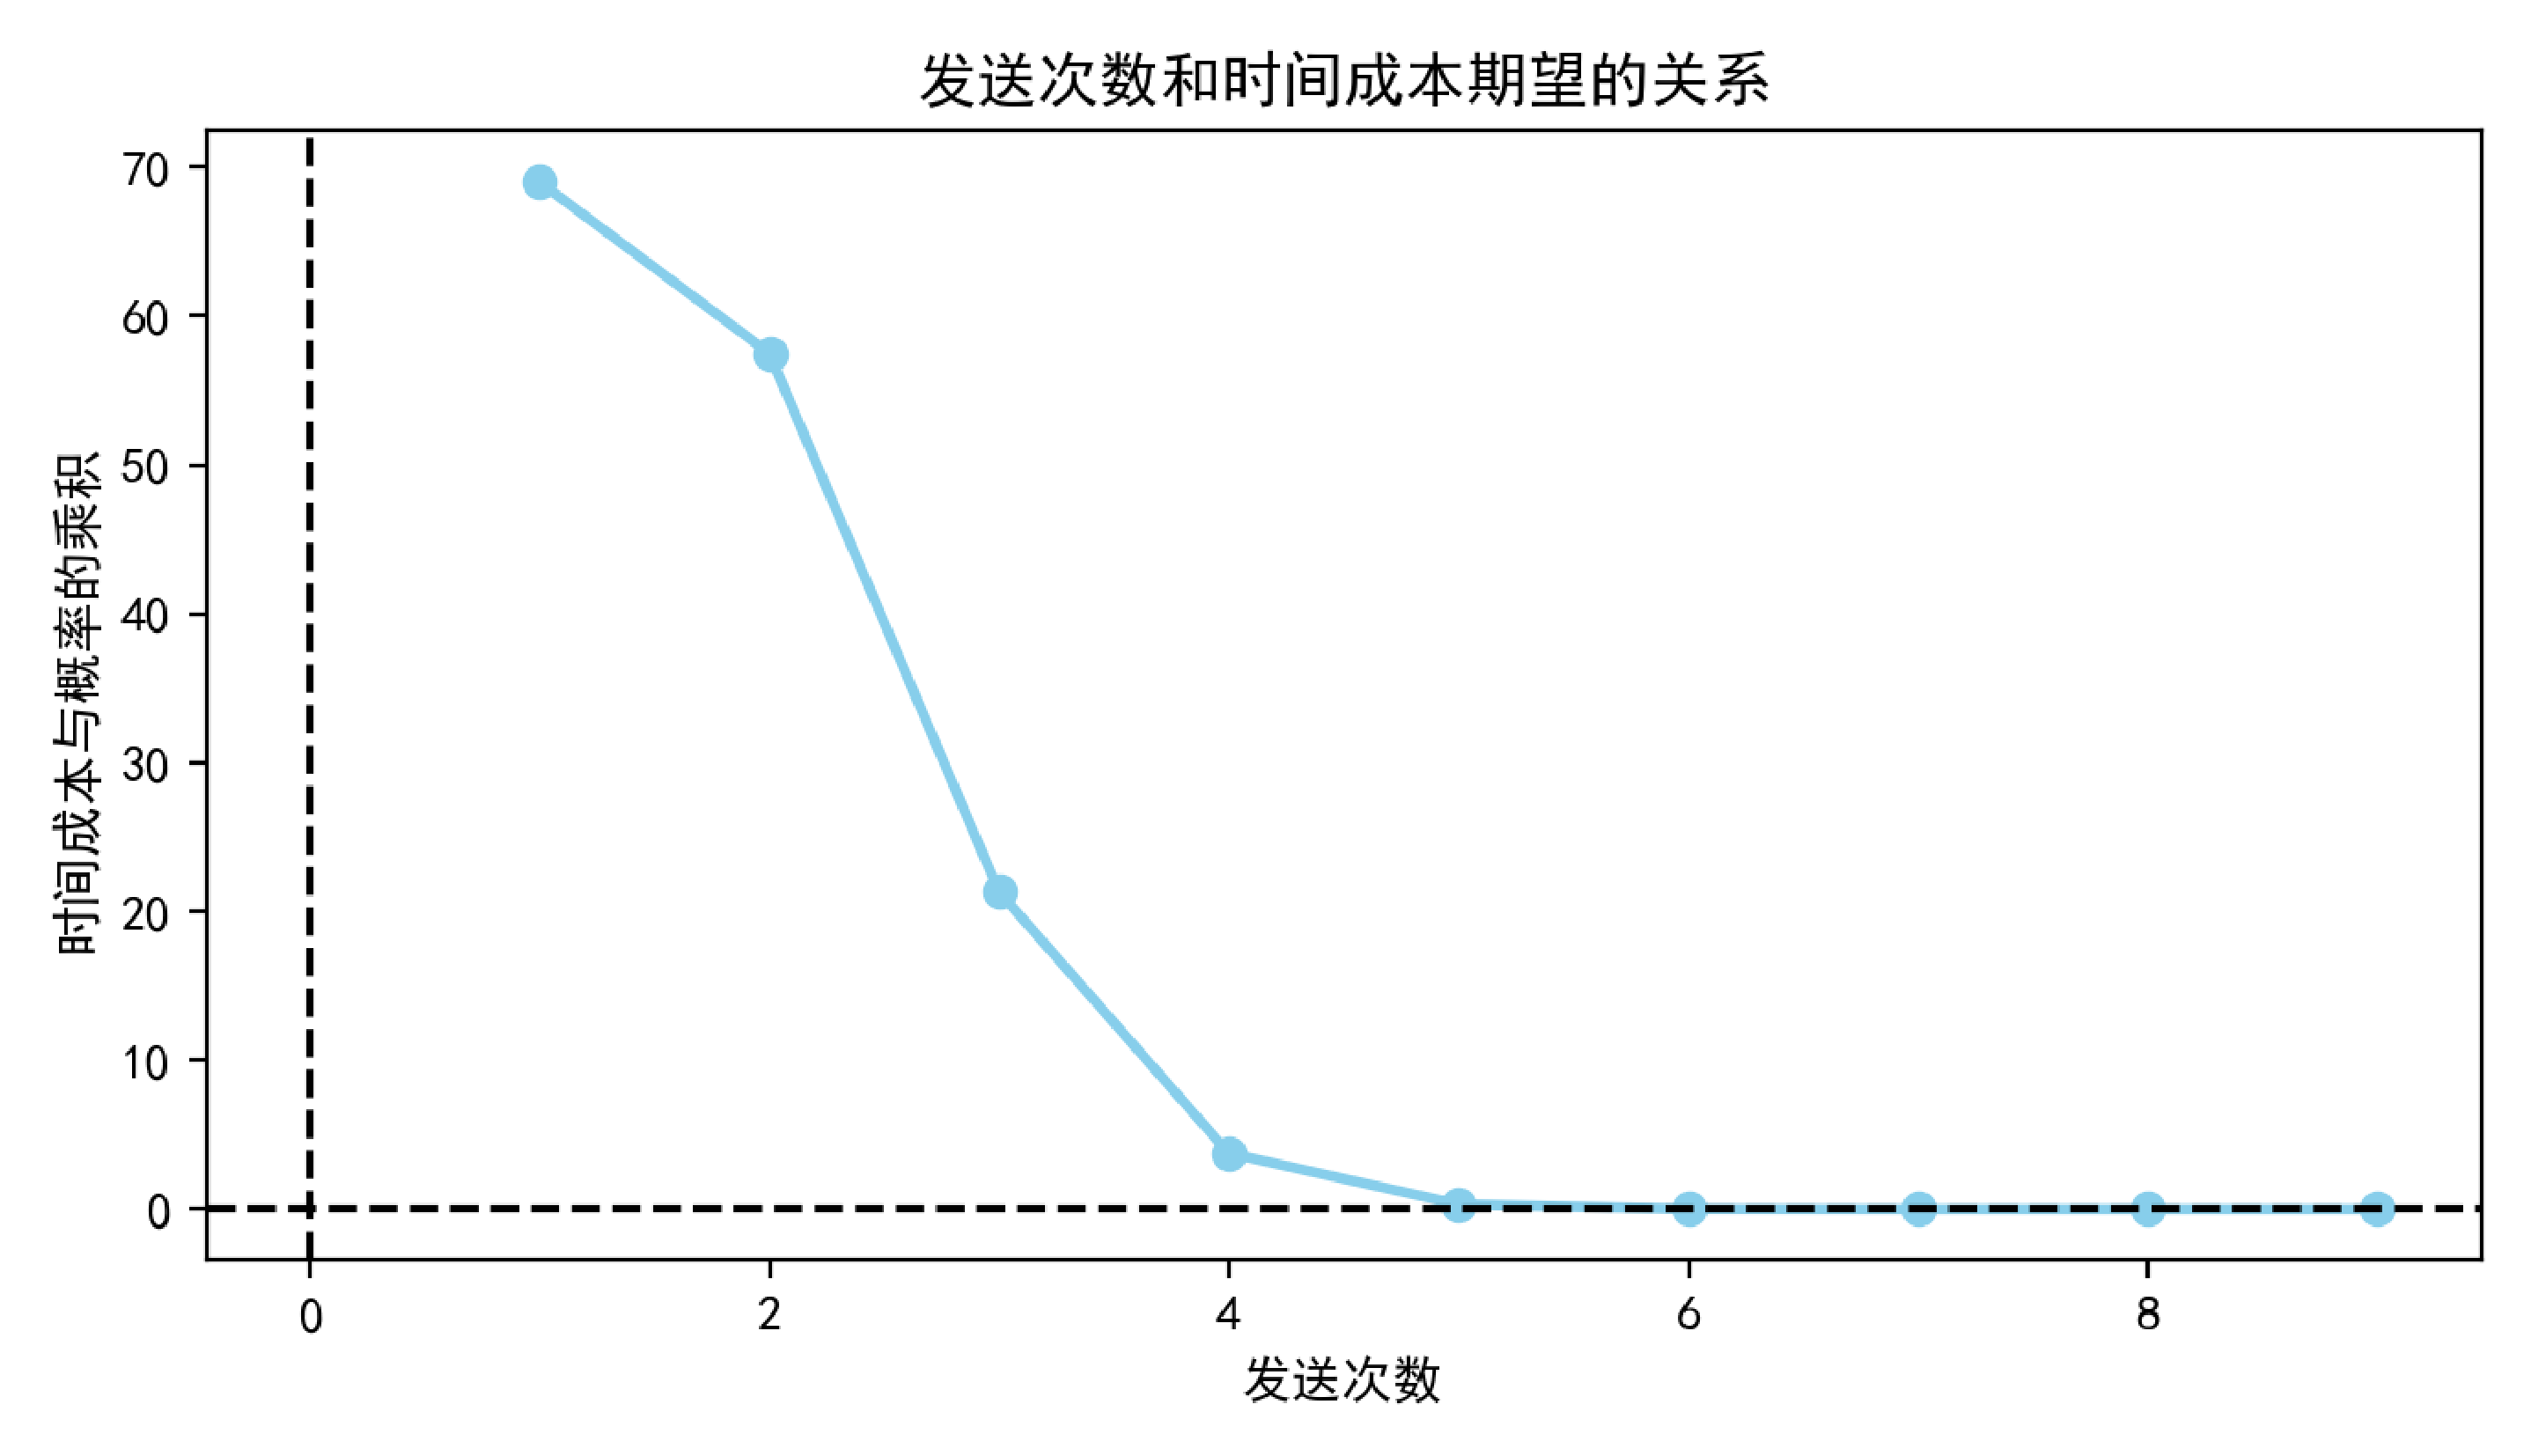
\includegraphics[width=0.75\linewidth]{figures/3}
	\caption{发送次数时间期望图($ap\_num=2,CW_{min}=6,CW_{max}=2100$)}
	\label{figure3}
\end{figure}

其再这种情形下,$ap\_num$为2,$CW_{min}$值为6,$CW_{max}$为2100个$slotTime$下,每次发送一个数据帧,所需等待时间151.9μs。

与随机回退机制息息相关的参数是per,丢包率这一项,丢包情况即不会收到确认帧情况,此时会让CW增加,以减少下一次发送数据冲突丢包。

\subsubsection{数据帧聚合策略分析}

在数据聚合策略中,存在两种聚合方式:ASMDU(A-MSDU Aggregation)和APMDU(A-MPDU Aggregation)。ASMDU在链路层进行聚合,而APMDU则在物理层实施。据相关资料指出,ASMDU聚合的上限通常由最大传输单元(MTU)和最大帧大小决定,其典型值为1500字节。根据802.11n标准,一个AMPDU的最大长度可达到65535字节。在数据集中,pkt\_len值为1500字节,即聚合前每一帧的数据长度,已达到ASMDU聚合的上限,因此无法采用ASMDU策略,只能选择APMDU策略。

多个PMDU(MAC Protocol Data Unit)通过聚合共享一个PHY(Physical Layer)头,以减少每次发送所必需的开销。换言之,每聚合一个数据帧,将减少一个PHY头的开销,PHY头在20MHz带宽中,大约需要传输20μs,而PHYRate最小为8.6Mbps,即最小的PHY头大约需要20*8.6=172bits=21.5bytes。然而,聚合需要进行0至3字节的填充对齐,其预期开销为1.5字节。此外,还需添加4字节的分隔符。因此,物理层每聚合一个PMDU,总体上最少可以减少16bytes花销。

故聚合次数越多,可以认为信道利用率越高,但是相应的per丢包率等也会增加,两者都会对吞吐量有很大的影响故并非聚合越多吞吐量越大。

在数据上体现聚合影响的参数就是ppdu\_dur,num\_ppdu,per这三个参数。

\subsection{问题三求解}
\subsubsection{特征构建}

根据题目与资料搜集可知,聚合过程会将多个数据包合并成一个,从而减少每个包的头部开销,提高有效负载的比例。合并数据包可以减少传输中的延迟和等待时间,少信道竞争,优化信道使用,进一步提升整体吞吐量。所以对于聚合过程相关参数需要进行进一步提取。特征如下:

\begin{itemize}
	\item num\_ppdu: 一个数据帧的聚合个数。一次测试里,统计每个数据帧的聚合个数,取平均值。通过与累计随机回退时间组合可以得到新的特征值减少的回退时间期望。
	\item ppdu\_dur (s): 一个数据帧的时长。一次测试里,统计每个数据帧的时长,取平均值。
\end{itemize}

但是这两个重要参数并不属于特征而是标签,所以团队借鉴问题二中应用过的方法,即双层预测的思想,先对num\_ppdu与ppdu\_dur进行预测,预测结果作为训练预测吞吐量模型的输入值,这样通过两级联完成新特征值对AP吞吐量的关联构建。

\subsubsection{模型的建立与求解}


本题预测方法依然选用stacking模型,但是预测策略有所不同。对于吞吐量预测,由先进行ppdu\_dur和num\_ppdu,还有per三个参数的预测,将预测结果作为输入进行预测最终的吞吐量。数据流向图如下:


\begin{figure}[H]
	\centering
	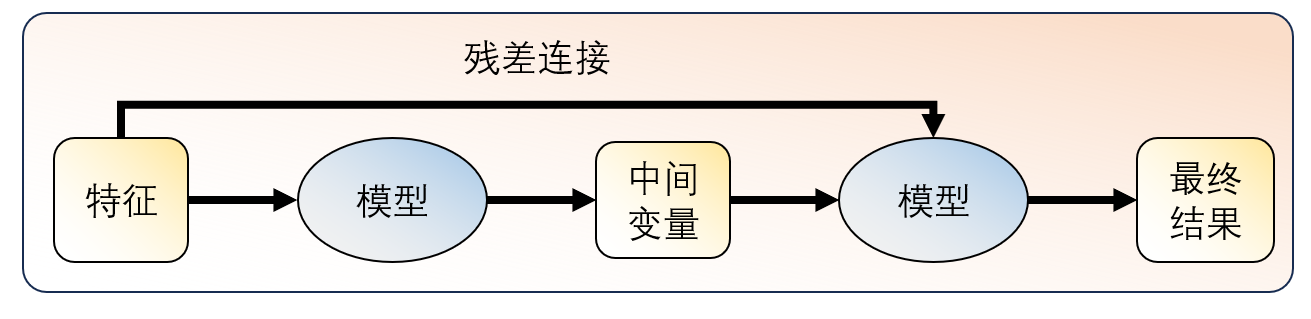
\includegraphics[width=0.7\linewidth]{figures/问题三流程}
	\caption{数据流向图}
	\label{fig:}
\end{figure}



基于以上分析,构建双层预测模型,上层预测输入特征值,输出目标变量num\_ppdu和ppdu\_dur;再将目标变量num\_ppdu和ppdu\_dur作为特征输入,构建吞吐量的下层预测模型。该层次预测模型所选用的上层特征如下表所示。

\begin{table}[H]
	\centering
	\caption{特征值(部分)}
	\begin{tabular}{ccccc} % 
		\toprule
		SINR & protocol & signal\_quality &  per & eirp\\ 
		\midrule
		30.064 & 20 & -72.2375 &  0.27 & 13 \\
		25 & 20 & -83.975 &  0.15 & 9 \\
		25 & 8 & -83.975 &  0.14 & 9 \\
		25.6628 & 20 & -83.8 &  0.17 & 10 \\
		43.6236 & 20 & -82.5389 &  0.03 & 10 \\
		\bottomrule
	\end{tabular}
\end{table}

上层预测模型输出num\_ppdu和ppdu\_dur后,同步更新下层输入特征,共计7类。经过5重交叉验证和网格搜索调参后,该层次预测模型的整体最优参数组合如下表所示。


\begin{table}[H]
	\centering
	\caption{最佳得分和参数设置}
	\begin{tabular}{cc}
		\toprule
		指标 & 最佳值/参数设置 \\
		\midrule
		最佳得分 (Best Score) & 0.8421 \\
		学习率 (Learning Rate) - 梯度提升 & 0.05 \\
		基学习器数量 (N\_estimators) - 梯度提升 & 100 \\
		最大深度 (Max Depth) - 随机森林 & 10 \\
		基学习器数量 (N\_estimators) - 随机森林 & 200 \\
		惩罚参数 (C) - 支持向量回归 & 10 \\
		核函数 (Kernel) - 支持向量回归 & `rbf' \\
		\bottomrule
	\end{tabular}
\end{table}


\begin{table}[H]
	\centering
	\caption{优化后的层次Stacking模型性能}
	\begin{tabular}{@{}cccc@{}}
		\toprule
		 均方误差 (MSE) & 均方根误差 (RMSE) & 平均绝对误差 (MAE) & 决定系数 (R²) \\
		\midrule
		 303.6069 & 17.4243 & 11.9287 & 0.9078 \\
		\bottomrule
	\end{tabular}
\end{table}

如表7.15所示,优化后的层次Stacking 模型在 MSE、RMSE 和 MAE 上表现良好,误差较小。同时,R² 值接近 1,显示出模型的高拟合度和解释能力。因此,该模型在处理吞吐量时具有很好的预测性能。

\begin{figure}[H]
	\centering
	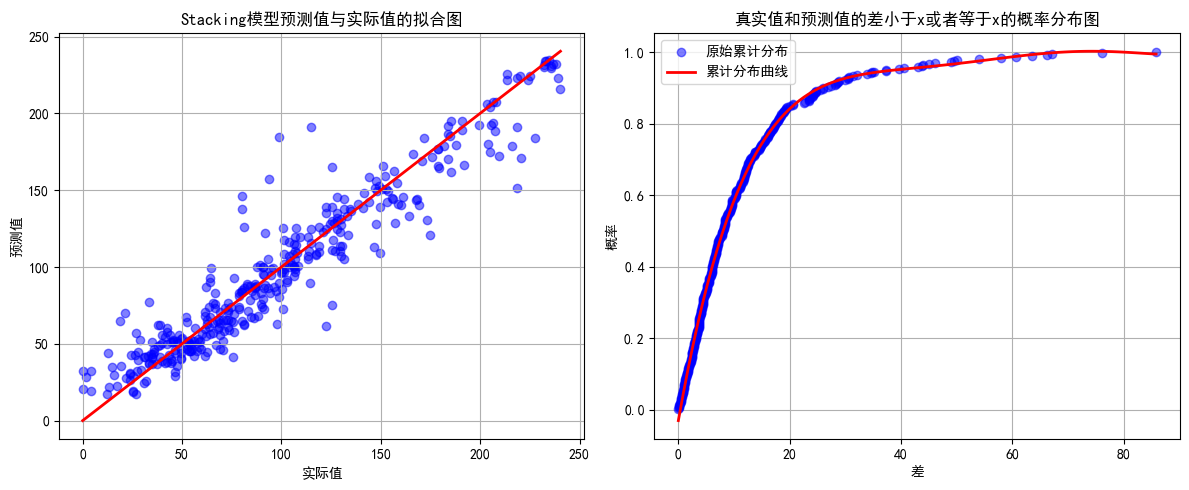
\includegraphics[width=0.8\linewidth]{figures/问题三888}
	\caption{模型预测性能图}
	\label{fig:888}
\end{figure}



如图7.19所示,层次Stacking 模型的残差分布近似正态分布,大量测试集的误差处于[ -10,+10 ]之间,平均绝对误差为11.9,稳定性较好,模型的预测精度较高。





\section{模型的评价与改进}
\subsection{模型的评价}

\begin{enumerate}
	\item 本文中构建的模型具有一定的灵活性,由于是对已有复杂的实测数据进行降维处理后,通过实际机理过程对数据进行二次加工,构建新特征作为模型的输入,保证了模型在数据上的灵活性以及模型的准确性。
	\item 本文中构建的模型具有一定的综合性,为了避免利用单一的学习器造成的过拟合情况,利用集成学习对数据进行二次学习,利用元学习器对最终数据进行学习并预测,通过网格搜索进行集成学习器的参数优化,提升模型的精度,并同时保持模型的综合性。
\end{enumerate}

\subsection{模型的改进}

\begin{enumerate}
	\item 在问题3分析中,对于随机回退机制的回退到0碰撞概率计算不严谨,在模型优化过程中,由于时间竞争窗口相关参数的缺失,导致模型对实际情况的预测不够精准。这一缺陷影响了模型在动态环境中对数据流量的准确把握,使得无法充分考虑竞争带来的延迟和数据丢失。因此,针对这一问题,我们需要改进模型结构,集成时间竞争窗口的相关参数,以更全面地反映系统的实时状态。这将增强模型在多任务环境中的适应性和预测能力,从而提升整体性能和准确性。
	
	\item 由于RSSI采样频率的限制,模型无法进行实时检测,从而可能导致数据延迟和信息缺失。这种情况会引发模型预测的误差,特别是在快速变化的环境中,无法准确捕捉到信号强度的动态变化。因此,为了改善这一问题,我们需要提高RSSI数据的采样频率,或引入更先进的数据插值和预测技术,以确保模型能够及时获取最新的信号信息。此外,结合时序数据分析方法,可以更好地捕捉到信号强度的变化趋势,从而提升模型的准确性和鲁棒性。通过这些改进,我们将能够更精确地反映实际信号环境,提高模型在复杂场景下的应用效果。
\end{enumerate}



\newpage

\begin{thebibliography}{9}
	
	\bibitem{reference1}
	王德营, 胡威, 吴通, 等. 基于Stacking集成学习的CANDU堆通道功率预测研究[J]. 核动力工程, 2024, 45(S1): 72-77. DOI: 10.13832/j.jnpe.2024.S1.0072.
	
	\bibitem{reference2}
	杨永鹏, 刘天琦, 杨真真. 一种基于IEEE 802.11ac协议标准的帧聚合实现算法[J]. 软件导刊, 2019, 18(09): 192-195.
	
	\bibitem{reference3}
	周海兴. 竞争窗口大小对IEEE 802.11无线网络的影响[J]. 广东通信技术, 2008, (10): 40-43+48.
	
	\bibitem{reference4}
	Yeh J H, Chen J C, Lee C C. WLAN standards[J]. IEEE Potentials, 2003, 22(4): 16-22.
	
	\bibitem{reference5}
	Muhammad Asif Khan, Ridha Hamila, Nasser Ahmed Al-Emadi, Serkan Kiranyaz, Moncef Gabbouj. Real-time throughput prediction for cognitive Wi-Fi networks[J]. Journal of Network and Computer Applications, Volume 150, 2020, 102499. ISSN 1084-8045.
	
\end{thebibliography}


%参考文献   手工录入
%\begin{thebibliography}{9}%宽度9
% \bibitem{bib:one} ....
% \bibitem{bib:two} ....
%\end{thebibliography}

%采用bibtex方案
\newpage

\appendix
\section{特征预处理代码}

\noindent 在本附录中,展示了用于特征预处理的 Python 代码。

\begin{lstlisting}
		# %% 特征预处理
	import pandas as pd
	# 读取 CSV 文件
	file_path = 'training_set_3ap_loc33_nav82.csv'
	data = pd.read_csv(file_path)
	
	# 提取第一行的 pd, ed, nav 和 pkt_len
	pd_, ed, nav, pk_len = data['pd'].iloc[0], data['ed'].iloc[0], data['nav'].iloc[0], data['pkt_len'].iloc[0]
	
	# 删除无关列
	data = data.drop(['test_dur', 'pd', 'ed', 'nav', 'loc_id', 'pkt_len', 'ap_name', 'ap_mac', 'sta_mac'], axis=1)
	
	# 将 ap_id 和 sta_id 转换为整数
	data['ap_id'] = data['ap_id'].str.replace('ap_', '').astype(int)
	data['sta_id'] = data['sta_id'].str.replace('sta_', '').astype(int)
	
	# 将协议映射为对应的数字
	data['protocol'] = data['protocol'].map({'tcp': 20 + 64, 'udp': 8})
	
	# 处理特定列的数据
	columns_to_process_ap = [col for col in data.columns if col.startswith('ap_from') or col.startswith('ap_to')]
	data_ = data[columns_to_process_ap].applymap(lambda x: eval(x) if isinstance(x, str) and x.startswith('[') else [])
	
	# 去除异常值的函数
	def remove_outliers(data):
	data = pd.Series(data)
	mean = np.mean(data)
	std = np.std(data)
	lower_bound = mean - 3 * std
	upper_bound = mean + 3 * std
	return [x for x in data if x >= lower_bound and x <= upper_bound]
	
	# 对特定列去除异常值
	for col in columns_to_process_ap:
	data_[col] = data_[col].apply(remove_outliers)
	
	# 处理列表并生成统计特征
	def process_list_to_stats(df, column_name):
	if 'sum' in column_name:
	df[column_name] = df[column_name].apply(
	lambda x: math.log10(sum(math.pow(10, item) for item in x) / len(x)) if len(x) > 0 else 0
	)
	df = df.rename(columns={column_name: column_name + '_mean'})
	# 其他处理...
	return df
	
	# 对每一列应用统计特征处理
	for col in columns_to_process_ap:
	data = process_list_to_stats(data, col)
	
	# 计算噪声特征
	columns_to_process_ap_sum_noise = [col for col in data.columns if col.startswith('ap_from_ap') and 'sum' in col]
	data['ap_from_other_ap_sum_rssi_noise'] = data[columns_to_process_ap_sum_noise].applymap(
	lambda x: math.pow(10, x) if x < -10 else pow(10, -99)
	).sum(axis=1).apply(math.log10)
\end{lstlisting}


\noindent 在本附录中,展示了用于随即回退机制的 Python 代码。

\begin{lstlisting}

# %% 随即回退分析
def P(n,ap_num,CWmin):
Pn=1
for i in range(1,n):
Pn*=(ap_num-1) / (CWmin* 2**i )
Pn*=(1-(ap_num-1)/(CWmin * 2**n))
return Pn
import numpy as np
times=10 #十次
times_try = np.arange(1,times)
Pns = np.array([round(P(n, 2, 6), 10) for n in times_try])

import matplotlib.pyplot as plt
plt.rcParams['font.family'] = 'SimHei' # 选择一个支持中文的字体
plt.rcParams['axes.unicode_minus'] = False # 正确显示负号
bars = plt.bar(times_try, Pns, width=0.2)  # 设置柱子的粗度为0.5
plt.xticks(times_try)  # 将x轴下标以整数形式显示
plt.xlabel('发送次数')
plt.ylabel('概率')
plt.title('发送次数概率分布图')
plt.axhline(y=0, color='k', linestyle='--')
plt.axvline(x=0, color='k', linestyle='--')
for bar in bars:
yval = bar.get_height()
plt.text(bar.get_x() + bar.get_width()/2-0.2, yval, round(yval, 2), va='bottom')
plt.show()

CWmin=6
slotTime=9 #9us
CWmax=2100 * slotTime
times_cost=np.array([min(CWmax ,(CWmin-1)*slotTime/2 *(2**n-1) ) for n in range(1,times)])
import matplotlib.pyplot as plt

plt.figure(figsize=(10, 6))
plt.plot(times_try, times_cost, color='skyblue', marker='o')
plt.xlabel('发送次数')
plt.ylabel('时间成本/μs')
plt.title('发送次数与时间成本的关系')
plt.axhline(y=0, color='k', linestyle='--')
plt.axvline(x=0, color='k', linestyle='--')
plt.grid(False)
plt.show()


plt.figure(figsize=(10, 6))
plt.plot(times_try, times_cost * Pns, color='skyblue', marker='o', linestyle='-', linewidth=2)  # 设置线的颜色、标记、样式和宽度
plt.xlabel('发送次数')
plt.ylabel('时间成本与概率的乘积')
plt.title('发送次数和时间成本期望的关系')
plt.axhline(y=0, color='k', linestyle='--')
plt.axvline(x=0, color='k', linestyle='--')
plt.grid(False)
plt.show()
np.sum(times_cost * Pns)
\end{lstlisting}


\section{问题一代码}

\noindent 在本附录中,展示了2AP的预测模型代码。

\begin{lstlisting}
# 定义文件夹路径
folder_path = Path(r'C:\Users\Shawn\Desktop\shumo\2024年中国研究生数学建模竞赛赛题\B题\2AP_cleaned_data')

# 初始化一个空的列表用于存储所有数据
dataframes = []

# 遍历文件夹中的所有CSV文件
for file_path in folder_path.glob('*.csv'):
data = pd.read_csv(file_path)
dataframes.append(data)

# 合并所有 DataFrame,保留所有列
combined_data = pd.concat(dataframes, ignore_index=True, sort=False)

# 保存到新的CSV文件
# combined_data.to_csv(r'C:\Users\Shawn\Desktop\shumo\2024年中国研究生数学建模竞赛赛题\B题\combined_ap2.csv', index=False)

# 删去不需要的列
columns_to_remove = [
'predict throughput', 'error%', 'bss_id', 'ap_name','sta_id','test_id',
'ap_from_other_ap_sum_rssi_noise', 'ap_from_other_ap_max_rssi_noise',
'ap_from_other_ap_mean_rssi_noise', 'sta_id', 'sta_to_ap_0_sum_ant_rssi_mean',
'sta_to_ap_0_max_ant_rssi_free_rate', 'sta_to_ap_0_mean_ant_rssi_free_rate',
'sta_to_ap_1_sum_ant_rssi_mean', 'sta_to_ap_1_max_ant_rssi_free_rate',

'sta_to_ap_1_mean_ant_rssi_free_rate', 'sta_from_ap_0_sum_ant_rssi_mean',
'sta_from_ap_0_max_ant_rssi_free_rate', 'sta_from_ap_0_mean_ant_rssi_free_rate',
'sta_from_ap_1_sum_ant_rssi_mean', 'sta_from_ap_1_max_ant_rssi_free_rate',
'sta_from_ap_1_mean_ant_rssi_free_rate', 'sta_from_other_sta_sum', 'num_ampdu',
'ppdu_dur', 'other_air_time', 'sta_from_ap_signal', 'sta_from_ap_noise',

'sta_to_ap_signal', 'sta_to_ap_noise', 'sta_from_ap_signal_max_free_rate',
'sta_from_ap_noise_max_free_rate', 'sta_to_ap_signal_max_free_rate',
'sta_to_ap_noise_max_free_rate', 'sta_from_ap_signal_mean_free_rate',
'sta_from_ap_noise_mean_free_rate', 'sta_to_ap_signal_mean_free_rate',
'sta_to_ap_noise_mean_free_rate',
]

combined_data = combined_data.drop(columns=columns_to_remove, errors='ignore')

# 计算相关系数矩阵
correlations = combined_data.corr()

# 获取 'seq_time' 与其他变量的相关性并排序
seq_time_correlations = correlations['seq_time'].sort_values(ascending=False)

print("影响强弱排序:")
print(seq_time_correlations[1:])


# 选择相关性最强的特征
top_correlated_features = seq_time_correlations.index[1:].tolist()

# 去掉 'throughput' 列
top_correlated_features = [feature for feature in top_correlated_features if feature != 'throughput']


# # 选择相关性最强的前9个变量(去掉相关性最强的一个变量)
# top_correlated_features = seq_time_correlations.index[1:].tolist()

# 选择相关性最强的特征作为模型输入
X = combined_data[top_correlated_features]
y = combined_data['seq_time']

# 分割训练集和测试集
X_train, X_test, y_train, y_test = train_test_split(X, y, test_size=0.3, random_state=42)

# 定义数据预处理器,数值特征标准化
numeric_transformer = StandardScaler()

# 创建预处理步骤
preprocessor = ColumnTransformer(
transformers=[
('num', numeric_transformer, top_correlated_features)
])

# 定义多个模型进行对比
models = {
	'Gradient Boosting': GradientBoostingRegressor(random_state=42),
	'Random Forest': RandomForestRegressor(random_state=42),
	'Support Vector Regressor': SVR(),
	'Linear Regression': LinearRegression()
}

# 初始化一个字典存储模型的性能指标
results = {}

# 遍历每个模型,训练并评估它们的性能
for model_name, model in models.items():
# 创建pipeline
pipeline = Pipeline([
('preprocessor', preprocessor),  # 数据预处理
('regressor', model)  # 使用模型
])

# 训练模型
pipeline.fit(X_train, y_train)

# 预测
y_pred = pipeline.predict(X_test)

# 计算误差和评价指标
mse = mean_squared_error(y_test, y_pred)
rmse = np.sqrt(mse)
mae = mean_absolute_error(y_test, y_pred)
r2 = r2_score(y_test, y_pred)

# 将结果存入字典
results[model_name] = {
	'MSE': mse,
	'RMSE': rmse,
	'MAE': mae,
	'R²': r2
}

# 将结果输出为DataFrame
results_df = pd.DataFrame(results).T
print(results_df)

# 使用Stacking集成学习模型
stacking_regressor = StackingRegressor(
estimators=[
('gb', GradientBoostingRegressor(random_state=42)),
('rf', RandomForestRegressor(random_state=42)),
('svr', SVR())
],
final_estimator=LinearRegression()
)

# 创建Stacking模型的pipeline
stacking_pipeline = Pipeline([
('preprocessor', preprocessor),  # 数据预处理
('stacking_regressor', stacking_regressor)  # 集成模型
])

# 训练Stacking模型
stacking_pipeline.fit(X_train, y_train)

# 预测
y_pred_stack = stacking_pipeline.predict(X_test)

# 计算Stacking模型的性能指标
mse_stack = mean_squared_error(y_test, y_pred_stack)
rmse_stack = np.sqrt(mse_stack)
mae_stack = mean_absolute_error(y_test, y_pred_stack)
r2_stack = r2_score(y_test, y_pred_stack)

# 输出Stacking模型的评价指标
print("\nStacking模型性能:")
print(f"MSE: {mse_stack}")
print(f"RMSE: {rmse_stack}")
print(f"MAE: {mae_stack}")
print(f"R²: {r2_stack}")

# 将Stacking模型的性能添加到结果中
results['Stacking Model'] = {
	'MSE': mse_stack,
	'RMSE': rmse_stack,
	'MAE': mae_stack,
	'R²': r2_stack
}

# 更新结果展示
results_df = pd.DataFrame(results).T
print(results_df)



# 参数调整和优化
param_grid = {
	'stacking_regressor__gb__n_estimators': [100, 200],
	'stacking_regressor__gb__learning_rate': [0.05, 0.3],
	'stacking_regressor__rf__n_estimators': [100, 200],
	'stacking_regressor__rf__max_depth': [5, 10],
	'stacking_regressor__svr__C': [0.1, 1, 10],
	'stacking_regressor__svr__kernel': ['linear', 'rbf']
}

grid_search = GridSearchCV(estimator=stacking_pipeline, param_grid=param_grid, cv=3, scoring='neg_mean_squared_error', verbose=2, n_jobs=-1)
grid_search.fit(X_train, y_train)
best_params = grid_search.best_params_
best_score = -grid_search.best_score_

print("\nBest Grid Search Score and Parameters:")
print(f"Best Score: {best_score}")
print(f"Best Parameters: {best_params}")

# 最佳参数模型评估
best_stacking_model = grid_search.best_estimator_
y_pred_best_stack = best_stacking_model.predict(X_test)
mse_best_stack = mean_squared_error(y_test, y_pred_best_stack)
rmse_best_stack = np.sqrt(mse_best_stack)
mae_best_stack = mean_absolute_error(y_test, y_pred_best_stack)
r2_best_stack = r2_score(y_test, y_pred_best_stack)

print("\nStacking最佳参数模型性能:")
print("\nOptimized Stacking Model Performance:")
print(f"MSE: {mse_best_stack}")
print(f"RMSE: {rmse_best_stack}")
print(f"MAE: {mae_best_stack}")
print(f"R²: {r2_best_stack}")











import joblib

# 将模型保存到磁盘
model_filename = '2AP_stacking_model.pkl'
joblib.dump(best_stacking_model, model_filename)

print(f"模型已保存至 {model_filename}")

\end{lstlisting}





\noindent 在本附录中,展示了3AP的预测模型代码。

\begin{lstlisting}
	# 定义文件夹路径
	folder_path = Path(r'C:\Users\Shawn\Desktop\shumo\2024年中国研究生数学建模竞赛赛题\B题\3AP_cleaned_data')
	
	# 初始化一个空的列表用于存储所有数据
	dataframes = []
	
	# 遍历文件夹中的所有CSV文件
	for file_path in folder_path.glob('*.csv'):
	data = pd.read_csv(file_path)
	dataframes.append(data)
	
	# 合并所有 DataFrame,保留所有列
	combined_data = pd.concat(dataframes, ignore_index=True, sort=False)
	
	# 添加 SINR 列
	combined_data['SINR'] = combined_data['sta_from_ap_signal'] - combined_data['sta_from_ap_noise']
	
	
	# 将结果保存到CSV文件
	combined_data.to_csv(r'C:\Users\Shawn\Desktop\shumo\2024年中国研究生数学建模竞赛赛题\B题\combined_ap3.csv', index=False)
	
	# 删去不需要的列
	columns_to_remove = [
	'predict throughput', 'error%', 'bss_id', 'ap_name','sta_id','test_id',
	'ap_from_other_ap_sum_rssi_noise', 'ap_from_other_ap_max_rssi_noise',
	'ap_from_other_ap_mean_rssi_noise', 'sta_id', 'sta_to_ap_0_sum_ant_rssi_mean',
	'sta_to_ap_0_max_ant_rssi_free_rate', 'sta_to_ap_0_mean_ant_rssi_free_rate',
	'sta_to_ap_1_sum_ant_rssi_mean', 'sta_to_ap_1_max_ant_rssi_free_rate',
	
	'sta_to_ap_1_mean_ant_rssi_free_rate', 'sta_from_ap_0_sum_ant_rssi_mean',
	'sta_from_ap_0_max_ant_rssi_free_rate', 'sta_from_ap_0_mean_ant_rssi_free_rate',
	'sta_from_ap_1_sum_ant_rssi_mean', 'sta_from_ap_1_max_ant_rssi_free_rate',
	'sta_from_ap_1_mean_ant_rssi_free_rate', 'sta_from_other_sta_sum', 'num_ampdu',
	'ppdu_dur', 'other_air_time', 'sta_from_ap_signal', 'sta_from_ap_noise',
	
	'sta_to_ap_signal', 'sta_to_ap_noise', 'sta_from_ap_signal_max_free_rate',
	'sta_from_ap_noise_max_free_rate', 'sta_to_ap_signal_max_free_rate',
	'sta_to_ap_noise_max_free_rate', 'sta_from_ap_signal_mean_free_rate',
	'sta_from_ap_noise_mean_free_rate', 'sta_to_ap_signal_mean_free_rate',
	'sta_to_ap_noise_mean_free_rate',
	
	'sta_to_ap_2_mean_ant_rssi_free_rate', 'sta_to_ap_2_max_ant_rssi_free_rate',
	'sta_to_ap_2_sum_ant_rssi_mean',           
	'sta_from_ap_2_max_ant_rssi_free_rate',    
	'sta_from_ap_2_sum_ant_rssi_mean',         
	'sta_from_ap_2_mean_ant_rssi_free_rate',
	]
	
	combined_data = combined_data.drop(columns=columns_to_remove, errors='ignore')
	
	# 计算相关系数矩阵
	correlations = combined_data.corr()
	
	# 获取 'seq_time' 与其他变量的相关性并排序
	seq_time_correlations = correlations['seq_time'].sort_values(ascending=False)
	
	print("影响强弱排序:")
	print(seq_time_correlations[1:])
	
	# 选择相关性最强的特征
	top_correlated_features = seq_time_correlations.index[1:].tolist()
	
	# 去掉 'throughput' 列
	top_correlated_features = [feature for feature in top_correlated_features if feature != 'throughput']
	
	
	# # 选择相关性最强的前9个变量(去掉相关性最强的一个变量)
	# top_correlated_features = seq_time_correlations.index[1:].tolist()
	
	# 选择相关性最强的特征作为模型输入
	X = combined_data[top_correlated_features]
	y = combined_data['seq_time']
	
	# 分割训练集和测试集
	X_train, X_test, y_train, y_test = train_test_split(X, y, test_size=0.3, random_state=42)
	
	# 定义数据预处理器,数值特征标准化
	numeric_transformer = StandardScaler()
	
	# 创建预处理步骤
	preprocessor = ColumnTransformer(
	transformers=[
	('num', numeric_transformer, top_correlated_features)
	])
	
	# 定义多个模型进行对比
	models = {
		'Gradient Boosting': GradientBoostingRegressor(random_state=42),
		'Random Forest': RandomForestRegressor(random_state=42),
		'Support Vector Regressor': SVR(),
		'Linear Regression': LinearRegression()
	}
	
	# 初始化一个字典存储模型的性能指标
	results = {}
	
	# 遍历每个模型,训练并评估它们的性能
	for model_name, model in models.items():
	# 创建pipeline
	pipeline = Pipeline([
	('preprocessor', preprocessor),  # 数据预处理
	('regressor', model)  # 使用模型
	])
	
	# 训练模型
	pipeline.fit(X_train, y_train)
	
	# 预测
	y_pred = pipeline.predict(X_test)
	
	# 计算误差和评价指标
	mse = mean_squared_error(y_test, y_pred)
	rmse = np.sqrt(mse)
	mae = mean_absolute_error(y_test, y_pred)
	r2 = r2_score(y_test, y_pred)
	
	# 将结果存入字典
	results[model_name] = {
		'MSE': mse,
		'RMSE': rmse,
		'MAE': mae,
		'R²': r2
	}
	
	# 将结果输出为DataFrame
	results_df = pd.DataFrame(results).T
	print(results_df)
	
	# 使用Stacking集成学习模型
	stacking_regressor = StackingRegressor(
	estimators=[
	('gb', GradientBoostingRegressor(random_state=42)),
	('rf', RandomForestRegressor(random_state=42)),
	('svr', SVR())
	],
	final_estimator=LinearRegression()
	)
	
	# 创建Stacking模型的pipeline
	stacking_pipeline = Pipeline([
	('preprocessor', preprocessor),  # 数据预处理
	('stacking_regressor', stacking_regressor)  # 集成模型
	])
	
	# 训练Stacking模型
	stacking_pipeline.fit(X_train, y_train)
	
	# 预测
	y_pred_stack = stacking_pipeline.predict(X_test)
	
	# 计算Stacking模型的性能指标
	mse_stack = mean_squared_error(y_test, y_pred_stack)
	rmse_stack = np.sqrt(mse_stack)
	mae_stack = mean_absolute_error(y_test, y_pred_stack)
	r2_stack = r2_score(y_test, y_pred_stack)
	
	# 输出Stacking模型的评价指标
	print("\nStacking模型性能:")
	print(f"MSE: {mse_stack}")
	print(f"RMSE: {rmse_stack}")
	print(f"MAE: {mae_stack}")
	print(f"R²: {r2_stack}")
	
	# 将Stacking模型的性能添加到结果中
	results['Stacking Model'] = {
		'MSE': mse_stack,
		'RMSE': rmse_stack,
		'MAE': mae_stack,
		'R²': r2_stack
	}
	
	# 更新结果展示
	results_df = pd.DataFrame(results).T
	print(results_df)
	
	
	# 参数调整和优化
	param_grid = {
		'stacking_regressor__gb__n_estimators': [100, 200],
		'stacking_regressor__gb__learning_rate': [0.05, 0.3],
		'stacking_regressor__rf__n_estimators': [100, 200],
		'stacking_regressor__rf__max_depth': [5, 10],
		'stacking_regressor__svr__C': [0.1, 1, 10],
		'stacking_regressor__svr__kernel': ['linear', 'rbf']
	}
	
	grid_search = GridSearchCV(estimator=stacking_pipeline, param_grid=param_grid, cv=3, scoring='neg_mean_squared_error', verbose=2, n_jobs=-1)
	grid_search.fit(X_train, y_train)
	best_params = grid_search.best_params_
	best_score = -grid_search.best_score_
	
	print("\nBest Grid Search Score and Parameters:")
	print(f"Best Score: {best_score}")
	print(f"Best Parameters: {best_params}")
	
	# 最佳参数模型评估
	best_stacking_model = grid_search.best_estimator_
	y_pred_best_stack = best_stacking_model.predict(X_test)
	mse_best_stack = mean_squared_error(y_test, y_pred_best_stack)
	rmse_best_stack = np.sqrt(mse_best_stack)
	mae_best_stack = mean_absolute_error(y_test, y_pred_best_stack)
	r2_best_stack = r2_score(y_test, y_pred_best_stack)
	
	print("\nStacking最佳参数模型性能:")
	print("\nOptimized Stacking Model Performance:")
	print(f"MSE: {mse_best_stack}")
	print(f"RMSE: {rmse_best_stack}")
	print(f"MAE: {mae_best_stack}")
	print(f"R²: {r2_best_stack}")
	
	
	
	
	
	# 可视化Stacking模型的预测结果
	plt.figure(figsize=(10, 6))
	
	# 1. 拟合线图(预测值 vs 实际值)
	plt.subplot(1, 3, 1)  # 调整为 1 行 3 列的图
	plt.scatter(y_test, y_pred_stack, alpha=0.5, color='blue')
	plt.plot([y_test.min(), y_test.max()], [y_test.min(), y_test.max()], color='red', lw=2)
	plt.xlabel('实际值')
	plt.ylabel('预测值')
	plt.title('Stacking模型预测值与实际值的拟合图')
	plt.grid(True)
	
	# 2. 残差图(残差 vs 预测值)
	plt.subplot(1, 3, 2)
	residuals = y_test - y_pred_stack
	plt.scatter(y_pred_stack, residuals, alpha=0.5, color='green')
	plt.axhline(0, color='red', lw=2)
	plt.xlabel('预测值')
	plt.ylabel('残差')
	plt.title('Stacking模型残差图')
	plt.grid(True)
	
	# 3. 预测值 vs 实际值的散点图
	plt.subplot(1, 3, 3)
	plt.scatter(range(len(y_test)), y_test, alpha=0.5, color='blue', label='实际值')
	plt.scatter(range(len(y_pred_stack)), y_pred_stack, alpha=0.5, color='orange', label='预测值')
	plt.xlabel('样本索引')
	plt.ylabel('seq_time')
	plt.title('Stacking模型预测值与实际值的散点图')
	plt.legend()
	plt.grid(True)
	
	# 调整布局并展示图形
	plt.tight_layout()
	plt.show()
	
	# 误差分布图
	plt.figure(figsize=(8, 5))
	sns.histplot(residuals, bins=30, kde=True, color='purple')
	plt.xlabel('残差')
	plt.ylabel('频率')
	plt.title('(b) 3AP')
	plt.grid(True)
	plt.show()
	
	import joblib
	
	# 将模型保存到磁盘
	model_filename = '3AP_stacking_model.pkl'
	joblib.dump(best_stacking_model, model_filename)
	
	print(f"模型已保存至 {model_filename}")
	
\end{lstlisting}




\section{问题二代码}
\noindent 在本附录中,展示了层次预测模型代码。

\begin{lstlisting}

	
	
	# 定义文件夹路径
	folder_path1 = Path(r'C:\Users\Shawn\Desktop\shumo\2024年中国研究生数学建模竞赛赛题\B题\2AP_cleaned_data')
	
	# 初始化一个空的列表用于存储所有数据
	dataframes1 = []
	
	# 遍历文件夹中的所有CSV文件
	for file_path1 in folder_path1.glob('*.csv'):
	data = pd.read_csv(file_path1)
	dataframes1.append(data)
	
	# 合并所有 DataFrame,保留所有列
	combined_data1 = pd.concat(dataframes1, ignore_index=True, sort=False)
	
	# 删去不需要的列
	columns_to_remove = [
	'predict throughput', 'error%', 'bss_id', 'ap_name','sta_id','test_id',
	'ap_from_other_ap_sum_rssi_noise', 'ap_from_other_ap_max_rssi_noise',
	'ap_from_other_ap_mean_rssi_noise', 'sta_id', 'sta_to_ap_0_sum_ant_rssi_mean',
	'sta_to_ap_0_max_ant_rssi_free_rate', 'sta_to_ap_0_mean_ant_rssi_free_rate',
	'sta_to_ap_1_sum_ant_rssi_mean', 'sta_to_ap_1_max_ant_rssi_free_rate',
	
	'sta_to_ap_1_mean_ant_rssi_free_rate', 'sta_from_ap_0_sum_ant_rssi_mean',
	'sta_from_ap_0_max_ant_rssi_free_rate', 'sta_from_ap_0_mean_ant_rssi_free_rate',
	'sta_from_ap_1_sum_ant_rssi_mean', 'sta_from_ap_1_max_ant_rssi_free_rate',
	'sta_from_ap_1_mean_ant_rssi_free_rate', 'sta_from_other_sta_sum', 'num_ampdu',
	'ppdu_dur', 'other_air_time', 'sta_from_ap_signal', 'sta_from_ap_noise',
	
	'sta_to_ap_signal', 'sta_to_ap_noise', 'sta_from_ap_signal_max_free_rate',
	'sta_from_ap_noise_max_free_rate', 'sta_to_ap_signal_max_free_rate',
	'sta_to_ap_noise_max_free_rate', 'sta_from_ap_signal_mean_free_rate',
	'sta_from_ap_noise_mean_free_rate', 'sta_to_ap_signal_mean_free_rate',
	'sta_to_ap_noise_mean_free_rate',
	
	'seq_time','throughput',
	]
	
	combined_data1 = combined_data1.drop(columns=columns_to_remove, errors='ignore')
	
	# 定义文件夹路径
	folder_path2 = Path(r'C:\Users\Shawn\Desktop\shumo\2024年中国研究生数学建模竞赛赛题\B题\3AP_cleaned_data')
	
	# 初始化一个空的列表用于存储所有数据
	dataframes2 = []
	
	# 遍历文件夹中的所有CSV文件
	for file_path2 in folder_path2.glob('*.csv'):
	data = pd.read_csv(file_path2)
	dataframes2.append(data)
	
	# 合并所有 DataFrame,保留所有列
	combined_data2 = pd.concat(dataframes2, ignore_index=True, sort=False)
	
	# 添加 SINR 列
	combined_data2['SINR'] = combined_data2['sta_from_ap_signal'] - combined_data2['sta_from_ap_noise']
	
	
	# 删去不需要的列
	columns_to_remove2 = [
	'predict throughput', 'error%', 'bss_id', 'ap_name','sta_id','test_id',
	'ap_from_other_ap_sum_rssi_noise', 'ap_from_other_ap_max_rssi_noise',
	'ap_from_other_ap_mean_rssi_noise', 'sta_id', 'sta_to_ap_0_sum_ant_rssi_mean',
	'sta_to_ap_0_max_ant_rssi_free_rate', 'sta_to_ap_0_mean_ant_rssi_free_rate',
	'sta_to_ap_1_sum_ant_rssi_mean', 'sta_to_ap_1_max_ant_rssi_free_rate',
	
	'sta_to_ap_1_mean_ant_rssi_free_rate', 'sta_from_ap_0_sum_ant_rssi_mean',
	'sta_from_ap_0_max_ant_rssi_free_rate', 'sta_from_ap_0_mean_ant_rssi_free_rate',
	'sta_from_ap_1_sum_ant_rssi_mean', 'sta_from_ap_1_max_ant_rssi_free_rate',
	'sta_from_ap_1_mean_ant_rssi_free_rate', 'sta_from_other_sta_sum', 'num_ampdu',
	'ppdu_dur', 'other_air_time', 'sta_from_ap_signal', 'sta_from_ap_noise',
	
	'sta_to_ap_signal', 'sta_to_ap_noise', 'sta_from_ap_signal_max_free_rate',
	'sta_from_ap_noise_max_free_rate', 'sta_to_ap_signal_max_free_rate',
	'sta_to_ap_noise_max_free_rate', 'sta_from_ap_signal_mean_free_rate',
	'sta_from_ap_noise_mean_free_rate', 'sta_to_ap_signal_mean_free_rate',
	'sta_to_ap_noise_mean_free_rate',
	
	'sta_to_ap_2_mean_ant_rssi_free_rate', 'sta_to_ap_2_max_ant_rssi_free_rate',
	'sta_to_ap_2_sum_ant_rssi_mean',           
	'sta_from_ap_2_max_ant_rssi_free_rate',    
	'sta_from_ap_2_sum_ant_rssi_mean',         
	'sta_from_ap_2_mean_ant_rssi_free_rate',
	
	'seq_time','throughput',
	]
	
	combined_data2 = combined_data2.drop(columns=columns_to_remove2, errors='ignore')
	
	# 合并AP2和AP3
	combined_data = pd.concat([combined_data1, combined_data2], ignore_index=True)
	combined_data = combined_data.dropna(axis=1, how='any')
	
	# 删除 nss 列值为 0 的行
	combined_data = combined_data[combined_data['nss'] != 0]
	
	# 计算 nss 列中值为 2 的数量
	count_nss_2 = (combined_data['nss'] == 2).sum()
	
	# 计算 nss 列的总数
	total_count = combined_data.shape[0]
	
	# 计算占比
	percentage_nss_2 = count_nss_2 / total_count * 100
	
	# 打印结果
	print(f"nss 列值为 2 的占比: {percentage_nss_2:.2f}%")
	
	
	
	# 计算相关系数矩阵
	correlations = combined_data.corr()
	
	# 获取 'nss' 与其他变量的相关性并排序
	MCS_correlations = correlations['nss'].sort_values(ascending=False)
	
	print("'nss' 与其他变量的影响强弱排序:")
	print(MCS_correlations[1:])
	
	# 选择相关性最强的特征
	top_correlated_features = MCS_correlations.index[1:].tolist()
	
	# 去掉 'throughput' 列
	top_correlated_features = [feature for feature in top_correlated_features if feature != 'throughput']
	
	# 选择相关性最强的特征作为模型输入
	X = combined_data[top_correlated_features]
	y = combined_data['nss']
	
	## 聚类欠采样:使用K-means对多数类样本进行聚类,然后从每个聚类中选择代表性样本
	# 选择nss值为2的多数类样本
	majority_class = combined_data[combined_data['nss'] == 2]
	minority_class = combined_data[combined_data['nss'] == 1]
	
	# 设定K-means聚类的簇数
	num_clusters = min(11, len(majority_class))  # 根据多数类样本的数量调整簇数
	
	# 对多数类样本进行K-means聚类
	kmeans = KMeans(n_clusters=num_clusters, random_state=42)
	majority_class['cluster'] = kmeans.fit_predict(majority_class.drop(columns='nss'))
	
	# 从每个簇中选择一个样本
	representative_samples = majority_class.groupby('cluster').apply(lambda x: x.sample(n=5)).reset_index(drop=True)
	
	
	# 合并代表性样本与少数类样本
	resampled_data = pd.concat([representative_samples, minority_class], ignore_index=True)
	
	# 删去 cluster 列
	resampled_data = resampled_data.drop(columns='cluster')
	
	# 特征和标签
	X = resampled_data.drop(columns='nss')
	y = resampled_data['nss']
	
	
	
	
	# 分割训练集和测试集
	X_train, X_test, y_train, y_test = train_test_split(X, y, test_size=0.3, random_state=42)
	
	# 定义数据预处理器,数值特征标准化
	numeric_transformer = StandardScaler()
	
	# 创建预处理步骤
	preprocessor = ColumnTransformer(
	transformers=[
	('num', numeric_transformer, top_correlated_features)
	])
	
	# 使用 SMOTE 进行过采样
	smote = SMOTE(k_neighbors=10,random_state=42)
	X_train_resampled, y_train_resampled = smote.fit_resample(X_train, y_train)
	
	# 定义多个分类模型进行对比
	models = {
		'Gradient Boosting': GradientBoostingClassifier(random_state=42),
		'Random Forest': RandomForestClassifier(random_state=42, class_weight='balanced'),
		'Support Vector Classifier': SVC(class_weight='balanced', probability=True),
		'Logistic Regression': LogisticRegression(class_weight='balanced')
	}
	
	# 初始化一个字典存储模型的性能指标
	results = {}
	
	# 遍历每个模型,训练并评估它们的性能
	for model_name, model in models.items():
	# 创建pipeline
	pipeline = Pipeline([
	('preprocessor', preprocessor),  # 数据预处理
	('classifier', model)  # 使用模型
	])
	
	# 训练模型
	pipeline.fit(X_train_resampled, y_train_resampled)
	
	# 预测
	y_pred = pipeline.predict(X_test)
	
	# 计算评价指标
	accuracy = accuracy_score(y_test, y_pred)
	f1 = f1_score(y_test, y_pred, average='weighted')
	precision = precision_score(y_test, y_pred, average='weighted')
	recall = recall_score(y_test, y_pred, average='weighted')
	
	# 将结果存入字典
	results[model_name] = {
		'Accuracy': accuracy,
		'F1 Score': f1,
		'Precision': precision,
		'Recall': recall
	}
	
	# 将结果输出为DataFrame
	results_df = pd.DataFrame(results).T
	print(results_df)
	
	# 使用Stacking集成学习模型
	stacking_classifier = StackingClassifier(
	estimators=[
	('gb', GradientBoostingClassifier(random_state=42)),
	('rf', RandomForestClassifier(random_state=42, class_weight='balanced')),
	('svc', SVC(probability=True, class_weight='balanced'))
	],
	final_estimator=LogisticRegression(class_weight='balanced')
	)
	
	# 创建Stacking模型的pipeline
	stacking_pipeline = Pipeline([
	('preprocessor', preprocessor),  # 数据预处理
	('stacking_classifier', stacking_classifier)  # 集成模型
	])
	
	# 训练Stacking模型
	stacking_pipeline.fit(X_train_resampled, y_train_resampled)
	
	# 预测
	y_pred_stack = stacking_pipeline.predict(X_test)
	
	# 计算Stacking模型的性能指标
	accuracy_stack = accuracy_score(y_test, y_pred_stack)
	f1_stack = f1_score(y_test, y_pred_stack, average='weighted')
	precision_stack = precision_score(y_test, y_pred_stack, average='weighted')
	recall_stack = recall_score(y_test, y_pred_stack, average='weighted')
	
	# 输出Stacking模型的评价指标
	print("\nStacking模型性能:")
	print(f"Accuracy: {accuracy_stack}")
	print(f"F1 Score: {f1_stack}")
	print(f"Precision: {precision_stack}")
	print(f"Recall: {recall_stack}")
	
	# 将Stacking模型的性能添加到结果中
	results['Stacking Model'] = {
		'Accuracy': accuracy_stack,
		'F1 Score': f1_stack,
		'Precision': precision_stack,
		'Recall': recall_stack
	}
	
	# 更新结果展示
	results_df = pd.DataFrame(results).T
	print(results_df)
	
	
	# 定义Stacking模型的参数网格
	param_grid_stacking = {
		'stacking_classifier__gb__n_estimators': [100, 200],
		'stacking_classifier__gb__learning_rate': [0.01, 0.1],
		'stacking_classifier__rf__n_estimators': [100, 200],
		'stacking_classifier__rf__max_features': ['auto', 'sqrt'],
		'stacking_classifier__svc__C': [1, 10],
		'stacking_classifier__final_estimator__C': [0.1, 1, 10],
		'stacking_classifier__final_estimator__penalty': ['l1', 'l2']
	}
	
	# 配置GridSearchCV
	grid_search_stacking = GridSearchCV(
	estimator=stacking_pipeline,
	param_grid=param_grid_stacking,
	scoring='accuracy',
	cv=3,
	verbose=1,
	n_jobs=-1
	)
	
	# 执行网格搜索
	grid_search_stacking.fit(X_train, y_train)
	
	# 获取最佳参数和评分
	print("Stacking模型最佳参数和评分:", grid_search_stacking.best_params_, grid_search_stacking.best_score_)
	
	# 更新Stacking模型在测试集上的性能评估
	y_pred_stack_best = grid_search_stacking.predict(X_test)
	accuracy_stack_best = accuracy_score(y_test, y_pred_stack_best)
	f1_stack_best = f1_score(y_test, y_pred_stack_best, average='weighted')
	precision_stack_best = precision_score(y_test, y_pred_stack_best, average='weighted')
	recall_stack_best = recall_score(y_test, y_pred_stack_best, average='weighted')
	
	# 输出优化后的Stacking模型性能
	print("\n优化后的Stacking模型性能:")
	print(f"Accuracy: {accuracy_stack_best}")
	print(f"F1 Score: {f1_stack_best}")
	print(f"Precision: {precision_stack_best}")
	print(f"Recall: {recall_stack_best}")
	
	# 将优化后的性能添加到结果中
	results['Optimized Stacking Model'] = {
		'Accuracy': accuracy_stack_best,
		'F1 Score': f1_stack_best,
		'Precision': precision_stack_best,
		'Recall': recall_stack_best
	}
	
	# 更新结果DataFrame并展示
	results_df = pd.DataFrame(results).T
	print(results_df)
	
	
	
	
	
	
	
	
	
	
	

	
	# 保存最优的集成模型
	joblib.dump(grid_search_stacking.best_estimator_, 'q2_nss_stacking_model.pkl')
	print("最优的集成模型已保存为 'q2_nss_stacking_model.pkl'")
\end{lstlisting}



\section{问题三代码}


\begin{lstlisting}
	
# 定义文件夹路径
folder_path1 = Path(r'C:\Users\Shawn\Desktop\shumo\2024年中国研究生数学建模竞赛赛题\B题\2AP_cleaned_data')

# 初始化一个空的列表用于存储所有数据
dataframes1 = []

# 遍历文件夹中的所有CSV文件
for file_path1 in folder_path1.glob('*.csv'):
data = pd.read_csv(file_path1)
dataframes1.append(data)

# 合并所有 DataFrame,保留所有列
combined_data1 = pd.concat(dataframes1, ignore_index=True, sort=False)

# 删去不需要的列
columns_to_remove = [
'predict throughput', 'error%', 'bss_id', 'ap_name','test_id','sta_id',#'ap_id',
# 'ap_from_other_ap_sum_rssi_noise', 'ap_from_other_ap_max_rssi_noise',
# 'ap_from_other_ap_mean_rssi_noise', 
'sta_id', 'sta_to_ap_0_sum_ant_rssi_mean',
'sta_to_ap_0_max_ant_rssi_free_rate', 'sta_to_ap_0_mean_ant_rssi_free_rate',
'sta_to_ap_1_sum_ant_rssi_mean', 'sta_to_ap_1_max_ant_rssi_free_rate',

'sta_to_ap_1_mean_ant_rssi_free_rate', 'sta_from_ap_0_sum_ant_rssi_mean',
'sta_from_ap_0_max_ant_rssi_free_rate', 'sta_from_ap_0_mean_ant_rssi_free_rate',
'sta_from_ap_1_sum_ant_rssi_mean', 'sta_from_ap_1_max_ant_rssi_free_rate',
'sta_from_ap_1_mean_ant_rssi_free_rate', 'sta_from_other_sta_sum', 'num_ampdu',
'ppdu_dur', 'other_air_time', 'sta_from_ap_signal', 'sta_from_ap_noise',

'sta_to_ap_signal', 'sta_to_ap_noise', 'sta_from_ap_signal_max_free_rate',
'sta_from_ap_noise_max_free_rate', 'sta_to_ap_signal_max_free_rate',
'sta_to_ap_noise_max_free_rate', 'sta_from_ap_signal_mean_free_rate',
'sta_from_ap_noise_mean_free_rate', 'sta_to_ap_signal_mean_free_rate',
'sta_to_ap_noise_mean_free_rate',
'seq_time',
]

combined_data1 = combined_data1.drop(columns=columns_to_remove, errors='ignore')


# 定义文件夹路径
folder_path2 = Path(r'C:\Users\Shawn\Desktop\shumo\2024年中国研究生数学建模竞赛赛题\B题\3AP_cleaned_data')

# 初始化一个空的列表用于存储所有数据
dataframes2 = []

# 遍历文件夹中的所有CSV文件
for file_path2 in folder_path2.glob('*.csv'):
data = pd.read_csv(file_path2)
dataframes2.append(data)

# 合并所有 DataFrame,保留所有列
combined_data2 = pd.concat(dataframes2, ignore_index=True, sort=False)

# 添加 SINR 列
combined_data2['SINR'] = combined_data2['sta_from_ap_signal'] - combined_data2['sta_from_ap_noise']


# 删去不需要的列
columns_to_remove2 = [
'predict throughput', 'error%', 'bss_id', 'ap_name','test_id','sta_id',#'ap_id',
# 'ap_from_other_ap_sum_rssi_noise', 'ap_from_other_ap_max_rssi_noise',
# 'ap_from_other_ap_mean_rssi_noise', 
'sta_id', 'sta_to_ap_0_sum_ant_rssi_mean',
'sta_to_ap_0_max_ant_rssi_free_rate', 'sta_to_ap_0_mean_ant_rssi_free_rate',
'sta_to_ap_1_sum_ant_rssi_mean', 'sta_to_ap_1_max_ant_rssi_free_rate',

'sta_to_ap_1_mean_ant_rssi_free_rate', 'sta_from_ap_0_sum_ant_rssi_mean',
'sta_from_ap_0_max_ant_rssi_free_rate', 'sta_from_ap_0_mean_ant_rssi_free_rate',
'sta_from_ap_1_sum_ant_rssi_mean', 'sta_from_ap_1_max_ant_rssi_free_rate',
'sta_from_ap_1_mean_ant_rssi_free_rate', 'sta_from_other_sta_sum', 'num_ampdu',
'ppdu_dur', 'other_air_time', 'sta_from_ap_signal', 'sta_from_ap_noise',

'sta_to_ap_signal', 'sta_to_ap_noise', 'sta_from_ap_signal_max_free_rate',
'sta_from_ap_noise_max_free_rate', 'sta_to_ap_signal_max_free_rate',
'sta_to_ap_noise_max_free_rate', 'sta_from_ap_signal_mean_free_rate',
'sta_from_ap_noise_mean_free_rate', 'sta_to_ap_signal_mean_free_rate',
'sta_to_ap_noise_mean_free_rate',

'sta_to_ap_2_mean_ant_rssi_free_rate', 'sta_to_ap_2_max_ant_rssi_free_rate',
'sta_to_ap_2_sum_ant_rssi_mean',           
'sta_from_ap_2_max_ant_rssi_free_rate',    
'sta_from_ap_2_sum_ant_rssi_mean',         
'sta_from_ap_2_mean_ant_rssi_free_rate',
'seq_time',
]

combined_data2 = combined_data2.drop(columns=columns_to_remove2, errors='ignore')

# # 合并AP2和AP3
# combined_data = pd.concat([combined_data1, combined_data2], axis=1, join='outer')
# combined_data = combined_data.dropna(axis=1, how='any')
combined_data = pd.concat([combined_data1, combined_data2], ignore_index=True)
# 删除 nss 列值为 0 的行
combined_data = combined_data[combined_data['nss'] != 0]

# 创建phy_rate映射字典
phy_rate_map = {
	(0, 1): 8.6,  (0, 2): 17.2,
	(1, 1): 17.2, (1, 2): 34.4,
	(2, 1): 25.8, (2, 2): 51.6,
	(3, 1): 34.4, (3, 2): 68.8,
	(4, 1): 51.6, (4, 2): 103.2,
	(5, 1): 68.8, (5, 2): 137.6,
	(6, 1): 77.4, (6, 2): 154.9,
	(7, 1): 86.0, (7, 2): 172.1,
	(8, 1): 103.2,(8, 2): 206.5,
	(9, 1): 114.7,(9, 2): 229.4,
	(10, 1): 129.0,(10, 2): 258.1,
	(11, 1): 143.4,(11, 2): 286.8
}

# 使用map方法将mcs和nss的组合映射到phy_rate
combined_data['phy_rate'] = combined_data.apply(lambda row: phy_rate_map.get((row['mcs'], row['nss']), None), axis=1)



# 计算相关系数矩阵
correlations = combined_data.corr()

# 获取 'throughput' 与其他变量的相关性并排序
throughput_correlations = correlations['throughput'].sort_values(ascending=False)

print(" 'throughput' 与其他变量的影响强弱排序:")
print(throughput_correlations[1:])

# 选择相关性最强的特征
top_correlated_features = throughput_correlations.index[1:].tolist()


# plt.figure(figsize=(12, 6))

# # 直方图
# sns.histplot(combined_data['throughput'], bins=30, kde=True, color='blue', stat='density', alpha=0.5)

# plt.title('Throughput Distribution')
# plt.xlabel('Throughput')
# plt.ylabel('Density')
# plt.grid(True)
# plt.show()



# 选择相关性最强的特征作为模型输入
X = combined_data[top_correlated_features]
y = combined_data['throughput']

# 分割训练集和测试集
X_train, X_test, y_train, y_test = train_test_split(X, y, test_size=0.3, random_state=42)

# 定义数据预处理器,数值特征标准化
numeric_transformer = StandardScaler()

# 创建预处理步骤
preprocessor = ColumnTransformer(
transformers=[
('num', numeric_transformer, top_correlated_features)
])

# 定义多个模型进行对比
models = {
	'Gradient Boosting': GradientBoostingRegressor(random_state=42),
	'Random Forest': RandomForestRegressor(random_state=42),
	'Support Vector Regressor': SVR(),
	'Linear Regression': LinearRegression()
}

# 初始化一个字典存储模型的性能指标
results = {}

# 遍历每个模型,训练并评估它们的性能
for model_name, model in models.items():
# 创建pipeline
pipeline = Pipeline([
('preprocessor', preprocessor),  # 数据预处理
('regressor', model)  # 使用模型
])

# 训练模型
pipeline.fit(X_train, y_train)

# 预测
y_pred = pipeline.predict(X_test)

# 计算误差和评价指标
mse = mean_squared_error(y_test, y_pred)
rmse = np.sqrt(mse)
mae = mean_absolute_error(y_test, y_pred)
r2 = r2_score(y_test, y_pred)

# 将结果存入字典
results[model_name] = {
	'MSE': mse,
	'RMSE': rmse,
	'MAE': mae,
	'R²': r2
}

# 将结果输出为DataFrame
results_df = pd.DataFrame(results).T
print(results_df)

# 使用Stacking集成学习模型
stacking_regressor = StackingRegressor(
estimators=[
('gb', GradientBoostingRegressor(random_state=42)),
('rf', RandomForestRegressor(random_state=42)),
('svr', SVR())
],
final_estimator=LinearRegression()
)

# 创建Stacking模型的pipeline
stacking_pipeline = Pipeline([
('preprocessor', preprocessor),  # 数据预处理
('stacking_regressor', stacking_regressor)  # 集成模型
])

# 训练Stacking模型
stacking_pipeline.fit(X_train, y_train)

# 预测
y_pred_stack = stacking_pipeline.predict(X_test)

# 计算Stacking模型的性能指标
mse_stack = mean_squared_error(y_test, y_pred_stack)
rmse_stack = np.sqrt(mse_stack)
mae_stack = mean_absolute_error(y_test, y_pred_stack)
r2_stack = r2_score(y_test, y_pred_stack)

# 输出Stacking模型的评价指标
print("\nStacking模型性能:")
print(f"MSE: {mse_stack}")
print(f"RMSE: {rmse_stack}")
print(f"MAE: {mae_stack}")
print(f"R²: {r2_stack}")

# 将Stacking模型的性能添加到结果中
results['Stacking Model'] = {
	'MSE': mse_stack,
	'RMSE': rmse_stack,
	'MAE': mae_stack,
	'R²': r2_stack
}

# 更新结果展示
results_df = pd.DataFrame(results).T
print(results_df)

# 参数调整和优化
param_grid = {
	'stacking_regressor__gb__n_estimators': [100, 200],
	'stacking_regressor__gb__learning_rate': [0.05, 0.3],
	'stacking_regressor__rf__n_estimators': [100, 200],
	'stacking_regressor__rf__max_depth': [5, 10],
	'stacking_regressor__svr__C': [0.1, 1, 10],
	'stacking_regressor__svr__kernel': ['linear', 'rbf']
}

grid_search = GridSearchCV(estimator=stacking_pipeline, param_grid=param_grid, cv=3, scoring='neg_mean_squared_error', verbose=2, n_jobs=-1)
grid_search.fit(X_train, y_train)
best_params = grid_search.best_params_
best_score = -grid_search.best_score_

print("\nBest Grid Search Score and Parameters:")
print(f"Best Score: {best_score}")
print(f"Best Parameters: {best_params}")

# 最佳参数模型评估
best_stacking_model = grid_search.best_estimator_
y_pred_best_stack = best_stacking_model.predict(X_test)
mse_best_stack = mean_squared_error(y_test, y_pred_best_stack)
rmse_best_stack = np.sqrt(mse_best_stack)
mae_best_stack = mean_absolute_error(y_test, y_pred_best_stack)
r2_best_stack = r2_score(y_test, y_pred_best_stack)

print("\nStacking最佳参数模型性能:")
print("\nOptimized Stacking Model Performance:")
print(f"MSE: {mse_best_stack}")
print(f"RMSE: {rmse_best_stack}")
print(f"MAE: {mae_best_stack}")
print(f"R²: {r2_best_stack}")

\end{lstlisting}





\end{document}
